\newpage
\section{Thực hiện bằng Python}

\textbf{Dữ liệu được thu thập từ Yahoo Finance với cổ phiếu MSFT (Microsoft Corporation), giai đoạn từ năm 2013 đến năm 2025.}

\subsection{Step 1: Thu thập dữ liệu}

Sử dụng thư viện \texttt{yfinance} để tải dữ liệu giá đóng cửa (Close Price) của cổ phiếu MSFT.

\begin{figure}[!htp]
    \centering
    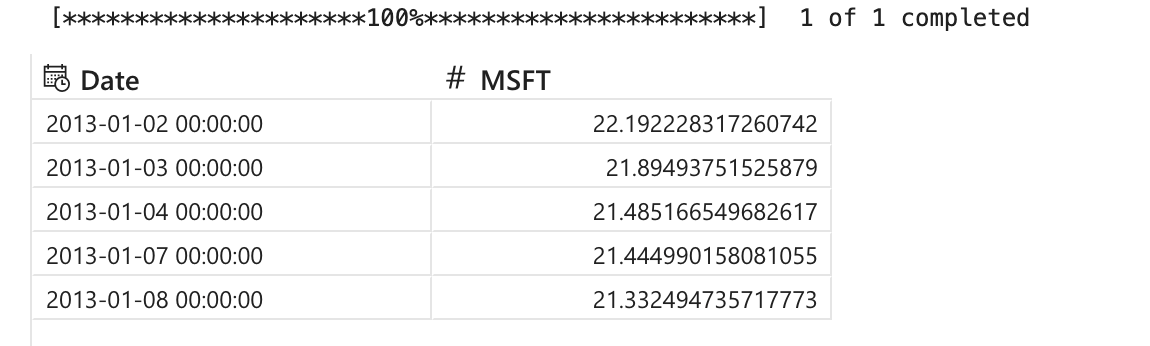
\includegraphics[width=0.95\textwidth]{LAB05/pics/step1_data.png}
    \caption{Dữ liệu giá đóng cửa MSFT}
\end{figure}

\subsection{Step 2: Trực quan hóa dữ liệu}

Vẽ biểu đồ chuỗi thời gian của giá cổ phiếu MSFT.

\begin{figure}[!htp]
    \centering
    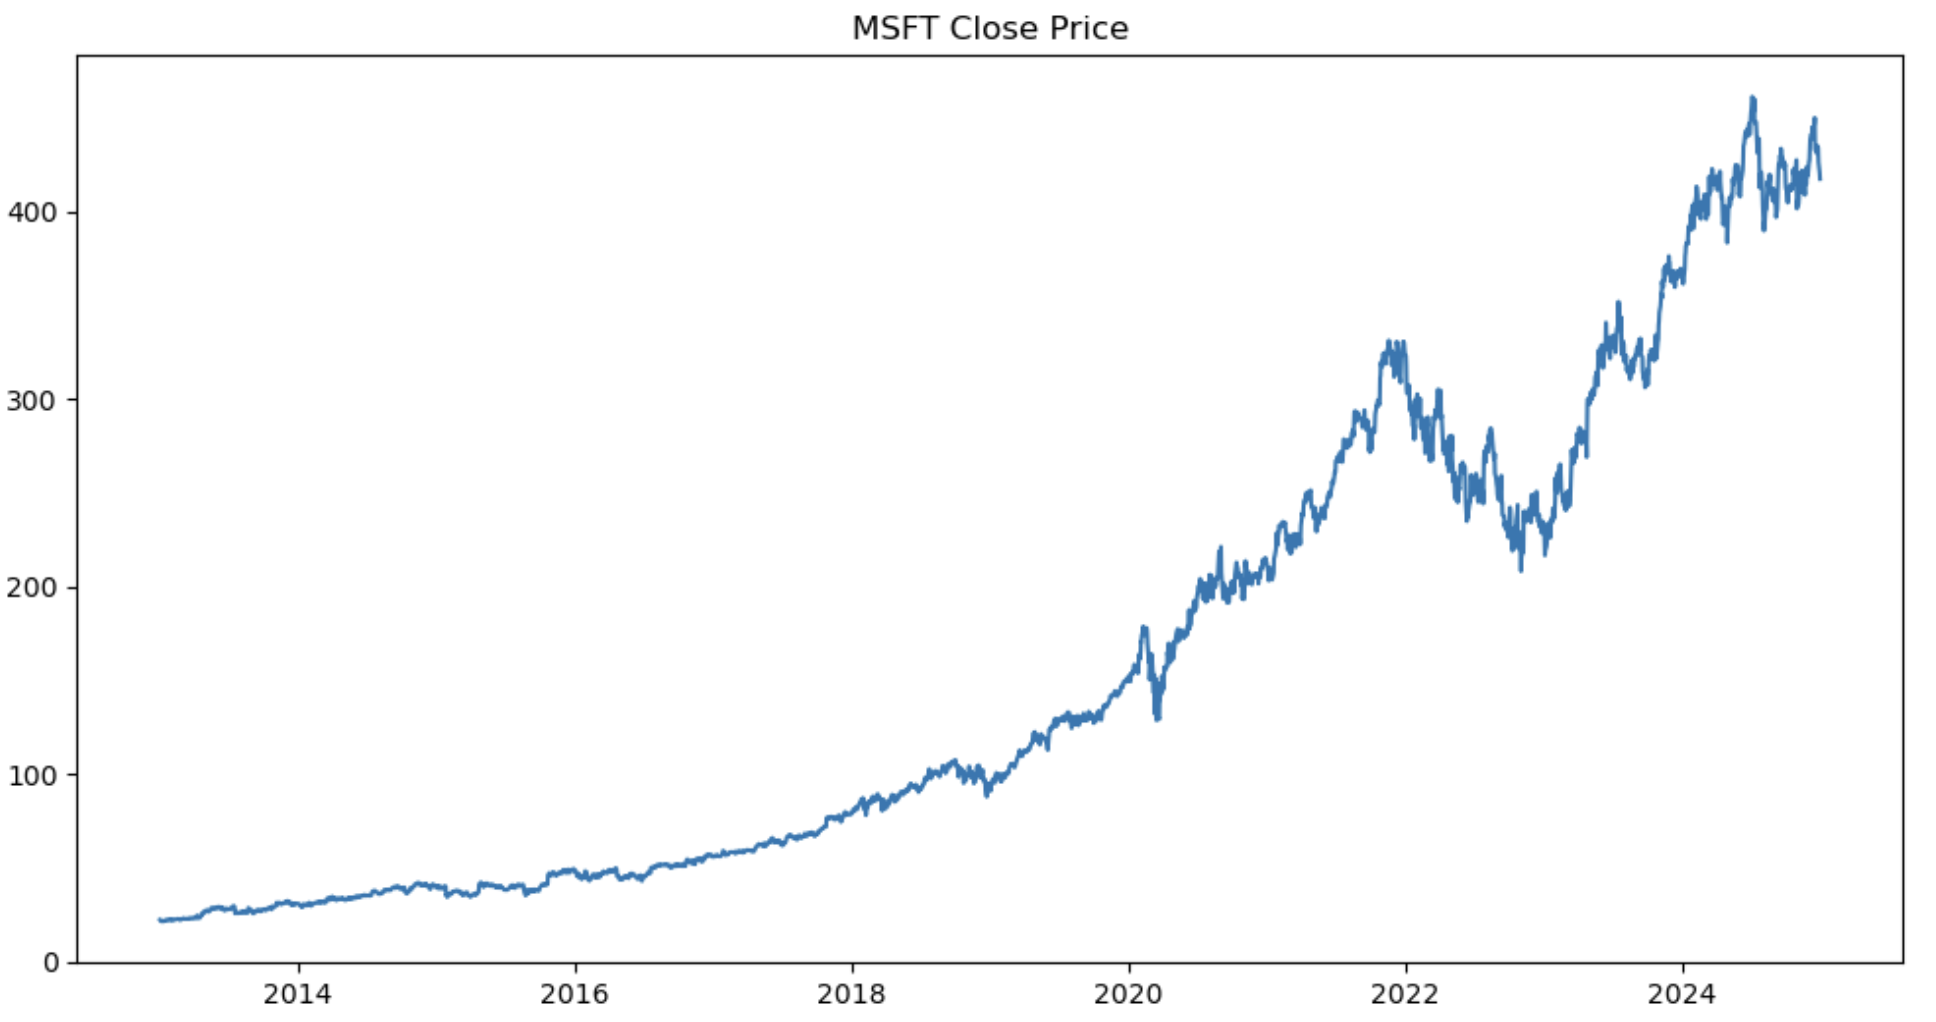
\includegraphics[width=0.95\textwidth]{LAB05/pics/step2_plot.png}
    \caption{Biểu đồ giá cổ phiếu MSFT}
\end{figure}

\textbf{Nhận xét:}
\begin{itemize}
    \item Dữ liệu có xu hướng tăng mạnh theo thời gian.
    \item Không thấy rõ tính mùa vụ.
    \item Giá trị trung bình thay đổi theo thời gian.
\end{itemize}

$\Rightarrow$ Chuỗi dữ liệu không có tính dừng (non-stationary).

\subsection{Step 3: Kiểm định ADF}

Sử dụng kiểm định Augmented Dickey-Fuller (ADF) để kiểm tra tính dừng của chuỗi.

\begin{figure}[!htp]
    \centering
    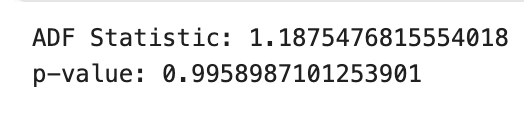
\includegraphics[width=0.6\textwidth]{LAB05/pics/step3_adf.png}
    \caption{Kết quả kiểm định ADF}
\end{figure}

\textbf{Kết luận:}
\begin{itemize}
    \item p-value > 0.05 $\Rightarrow$ không bác bỏ $H_0$
    \item Chuỗi không dừng
\end{itemize}

\subsection{Step 4: Sai phân dữ liệu}

Tiến hành sai phân bậc 1 để làm chuỗi trở nên dừng.

\begin{figure}[!htp]
    \centering
    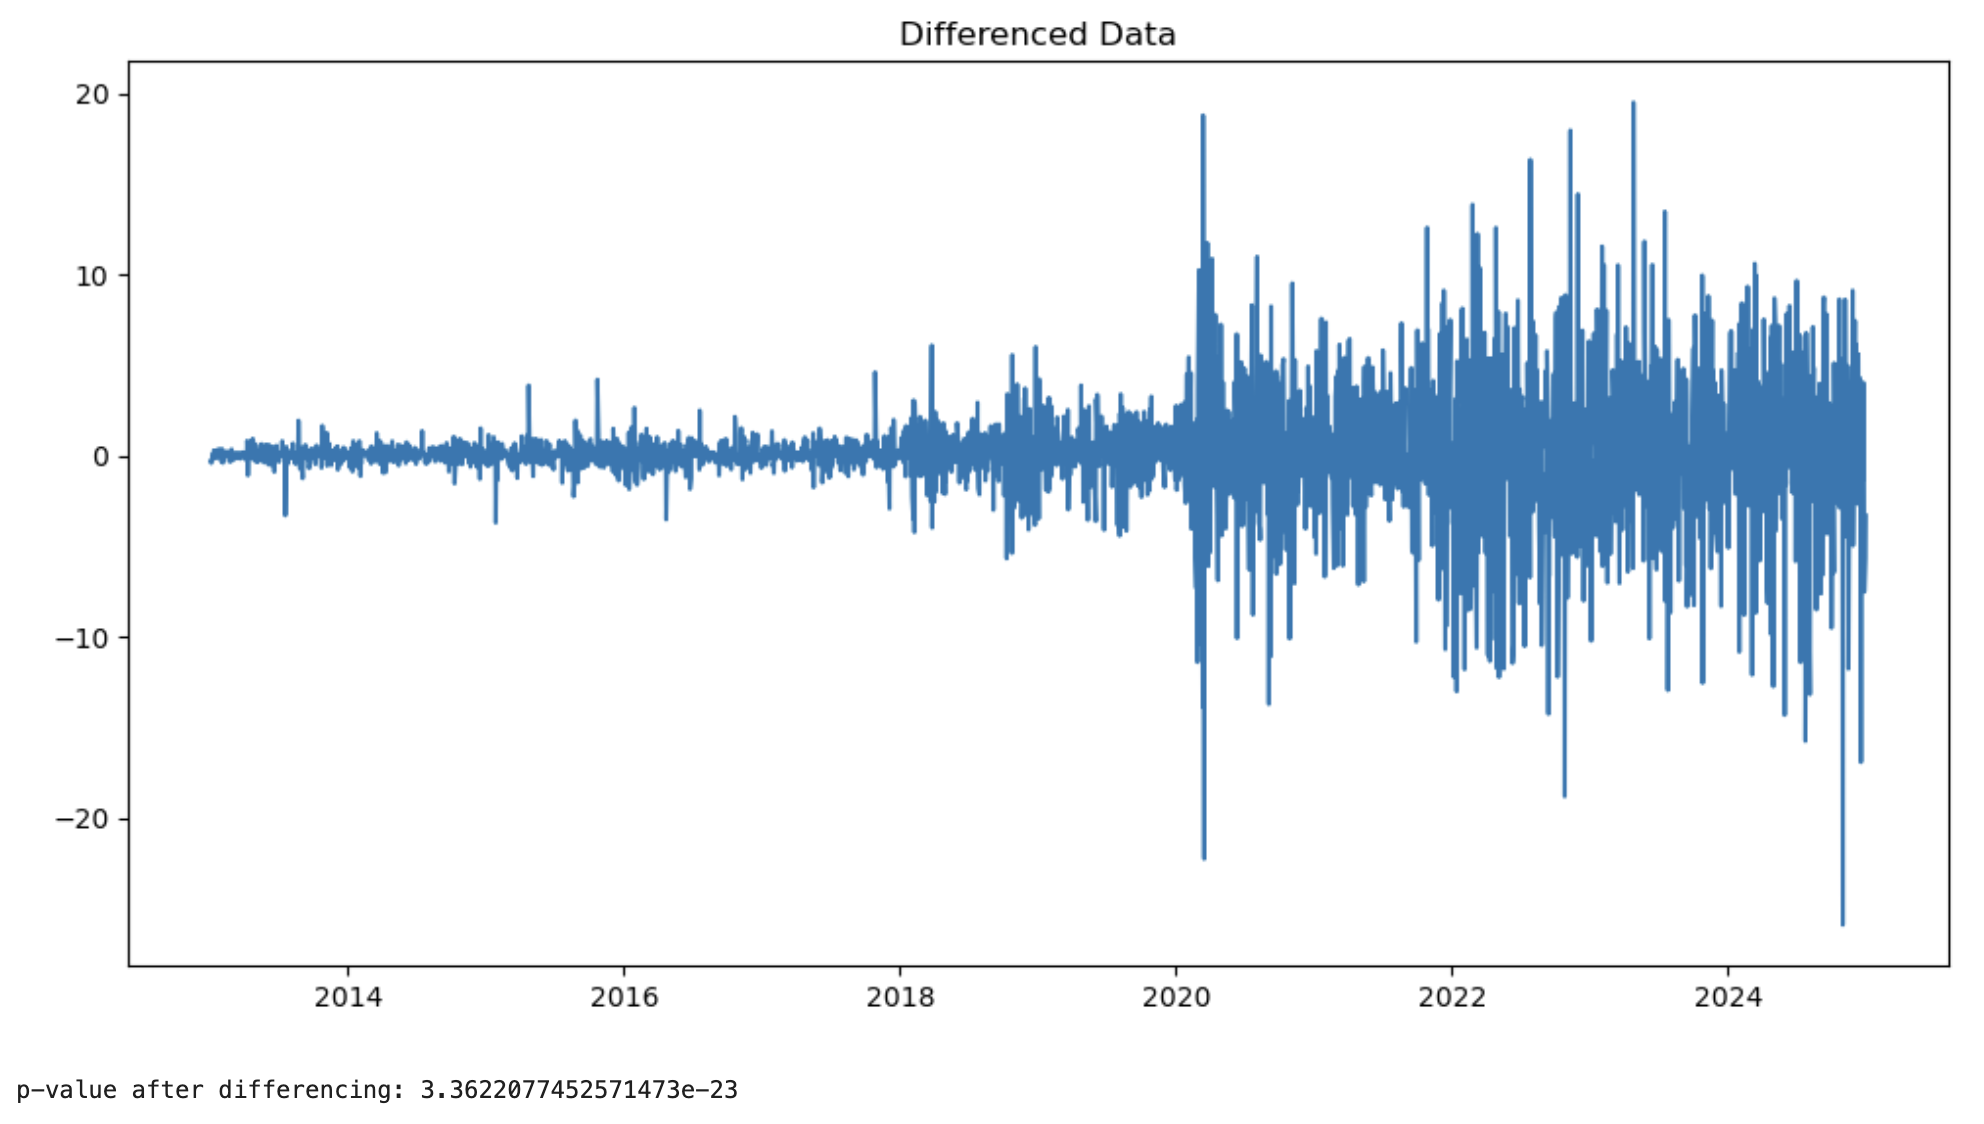
\includegraphics[width=0.95\textwidth]{LAB05/pics/step4_diff.png}
    \caption{Chuỗi sau khi sai phân}
\end{figure}

Sau khi sai phân, kiểm định ADF cho thấy p-value < 0.05 $\Rightarrow$ chuỗi dừng.

$\Rightarrow$ Chọn $d = 1$

\subsection{Step 5: Xác định tham số p và q}

Sử dụng biểu đồ ACF và PACF để xác định tham số.

\begin{figure}[!htp]
    \centering
    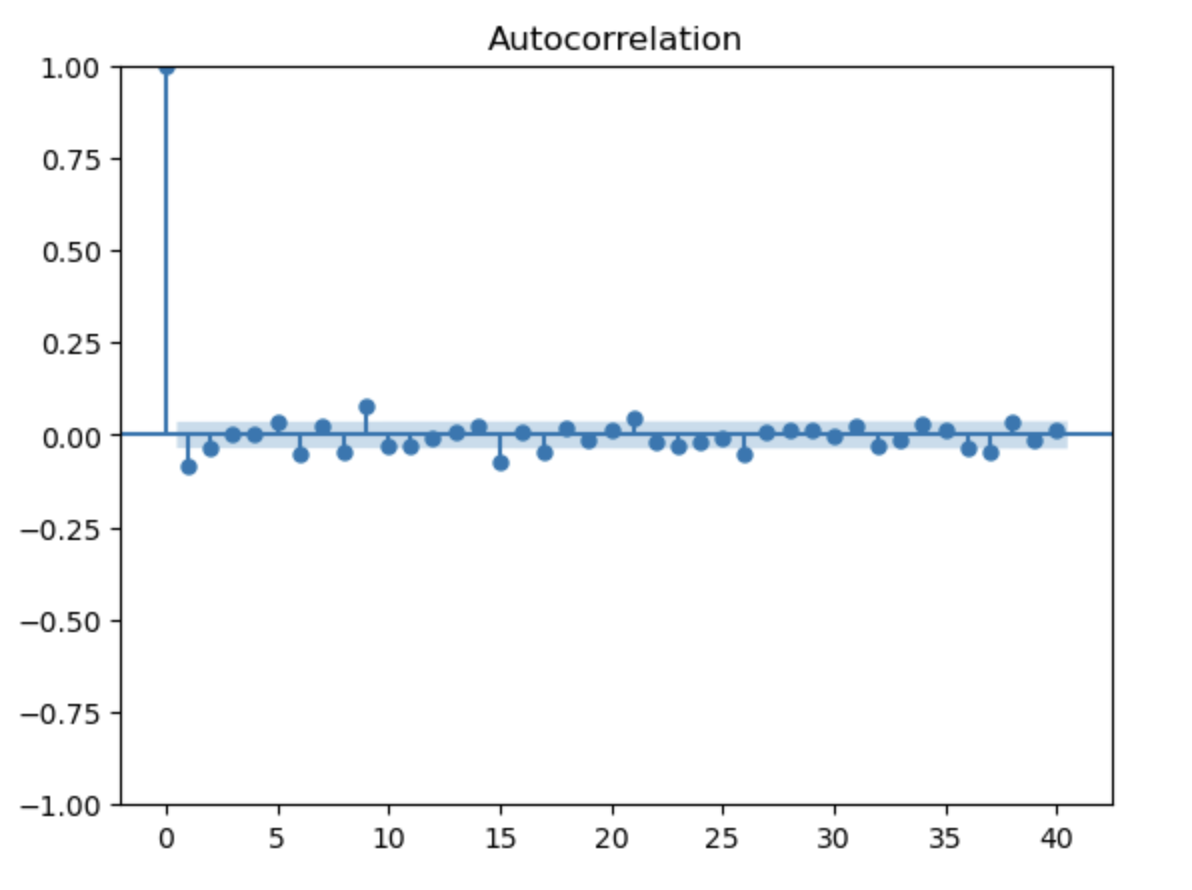
\includegraphics[width=0.95\textwidth]{LAB05/pics/step5_acf.png}
    \caption{Biểu đồ ACF}
\end{figure}

\begin{figure}[!htp]
    \centering
    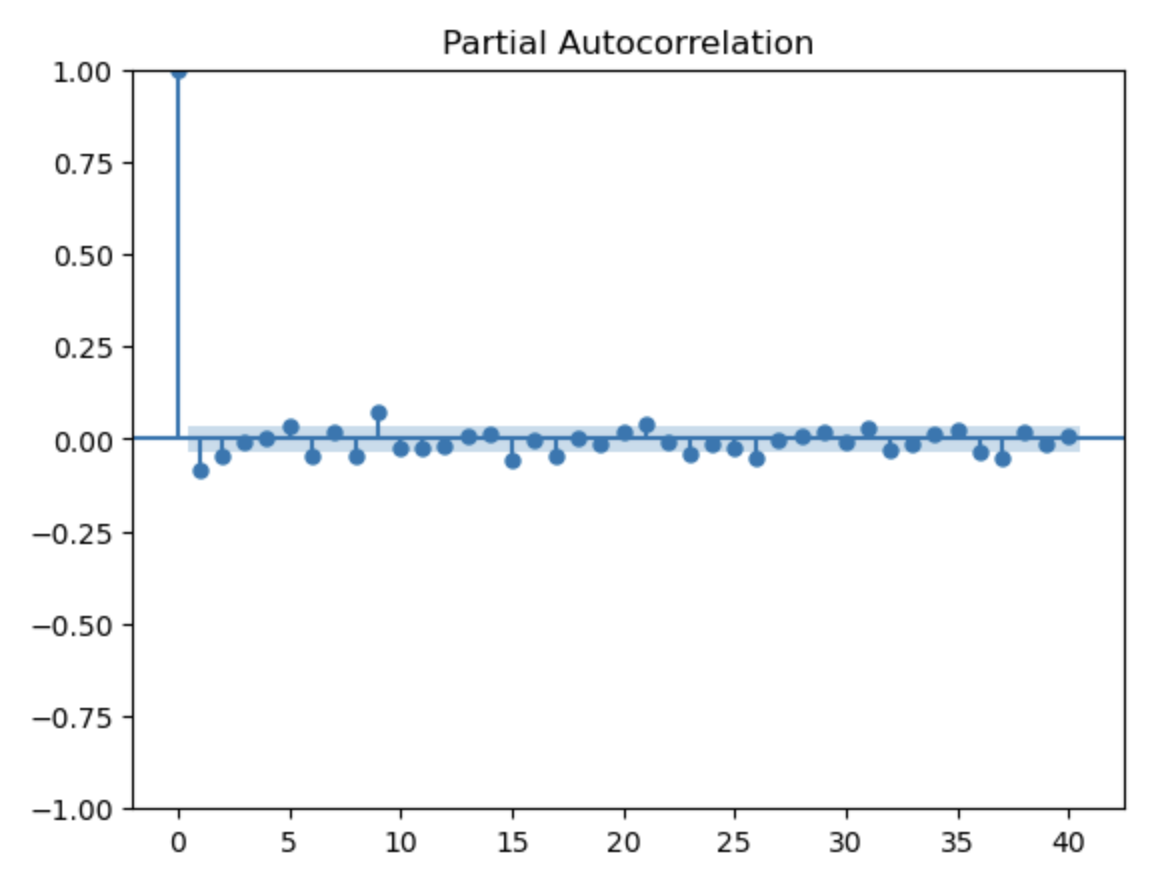
\includegraphics[width=0.95\textwidth]{LAB05/pics/step5_pacf.png}
    \caption{Biểu đồ PACF}
\end{figure}

\textbf{Nhận xét:}
\begin{itemize}
    \item PACF cắt tại lag 1 $\Rightarrow$ chọn $p = 1$
    \item ACF cắt tại lag 1 $\Rightarrow$ chọn $q = 1$
\end{itemize}

$\Rightarrow$ Mô hình ban đầu: \textbf{ARIMA(1,1,1)}

\subsection{Step 6: Xây dựng mô hình}

Xây dựng mô hình ARIMA(1,1,1) trên tập train.

\begin{figure}[!htp]
    \centering
    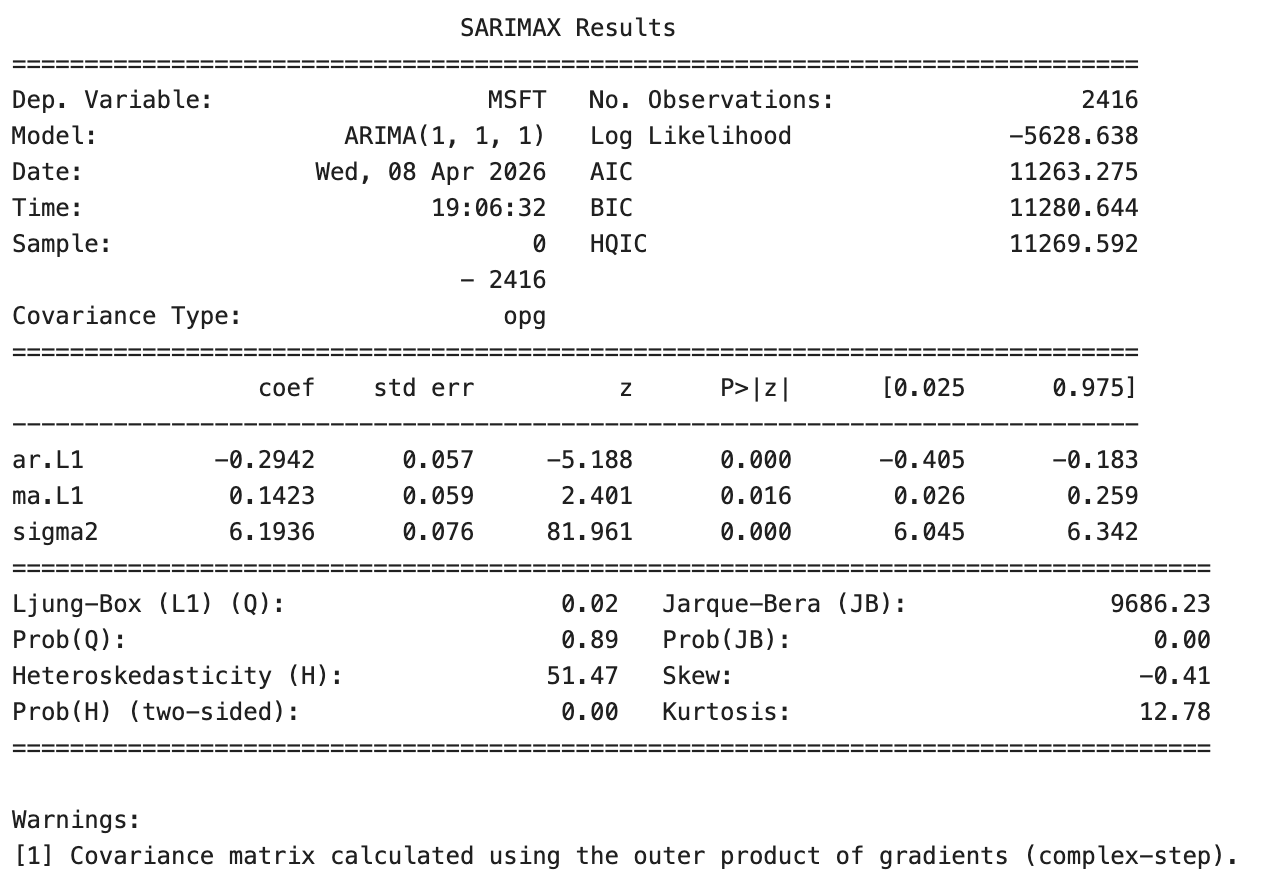
\includegraphics[width=0.95\textwidth]{LAB05/pics/step6_model.png}
    \caption{Kết quả ước lượng mô hình ARIMA}
\end{figure}

\textbf{Nhận xét:}
\begin{itemize}
    \item Các hệ số AR và MA có ý nghĩa thống kê (p-value < 0.05)
    \item Mô hình phù hợp về mặt lý thuyết
\end{itemize}

\subsection{Step 7: Dự báo}

Thực hiện dự báo trên tập test.

\begin{figure}[!htp]
    \centering
    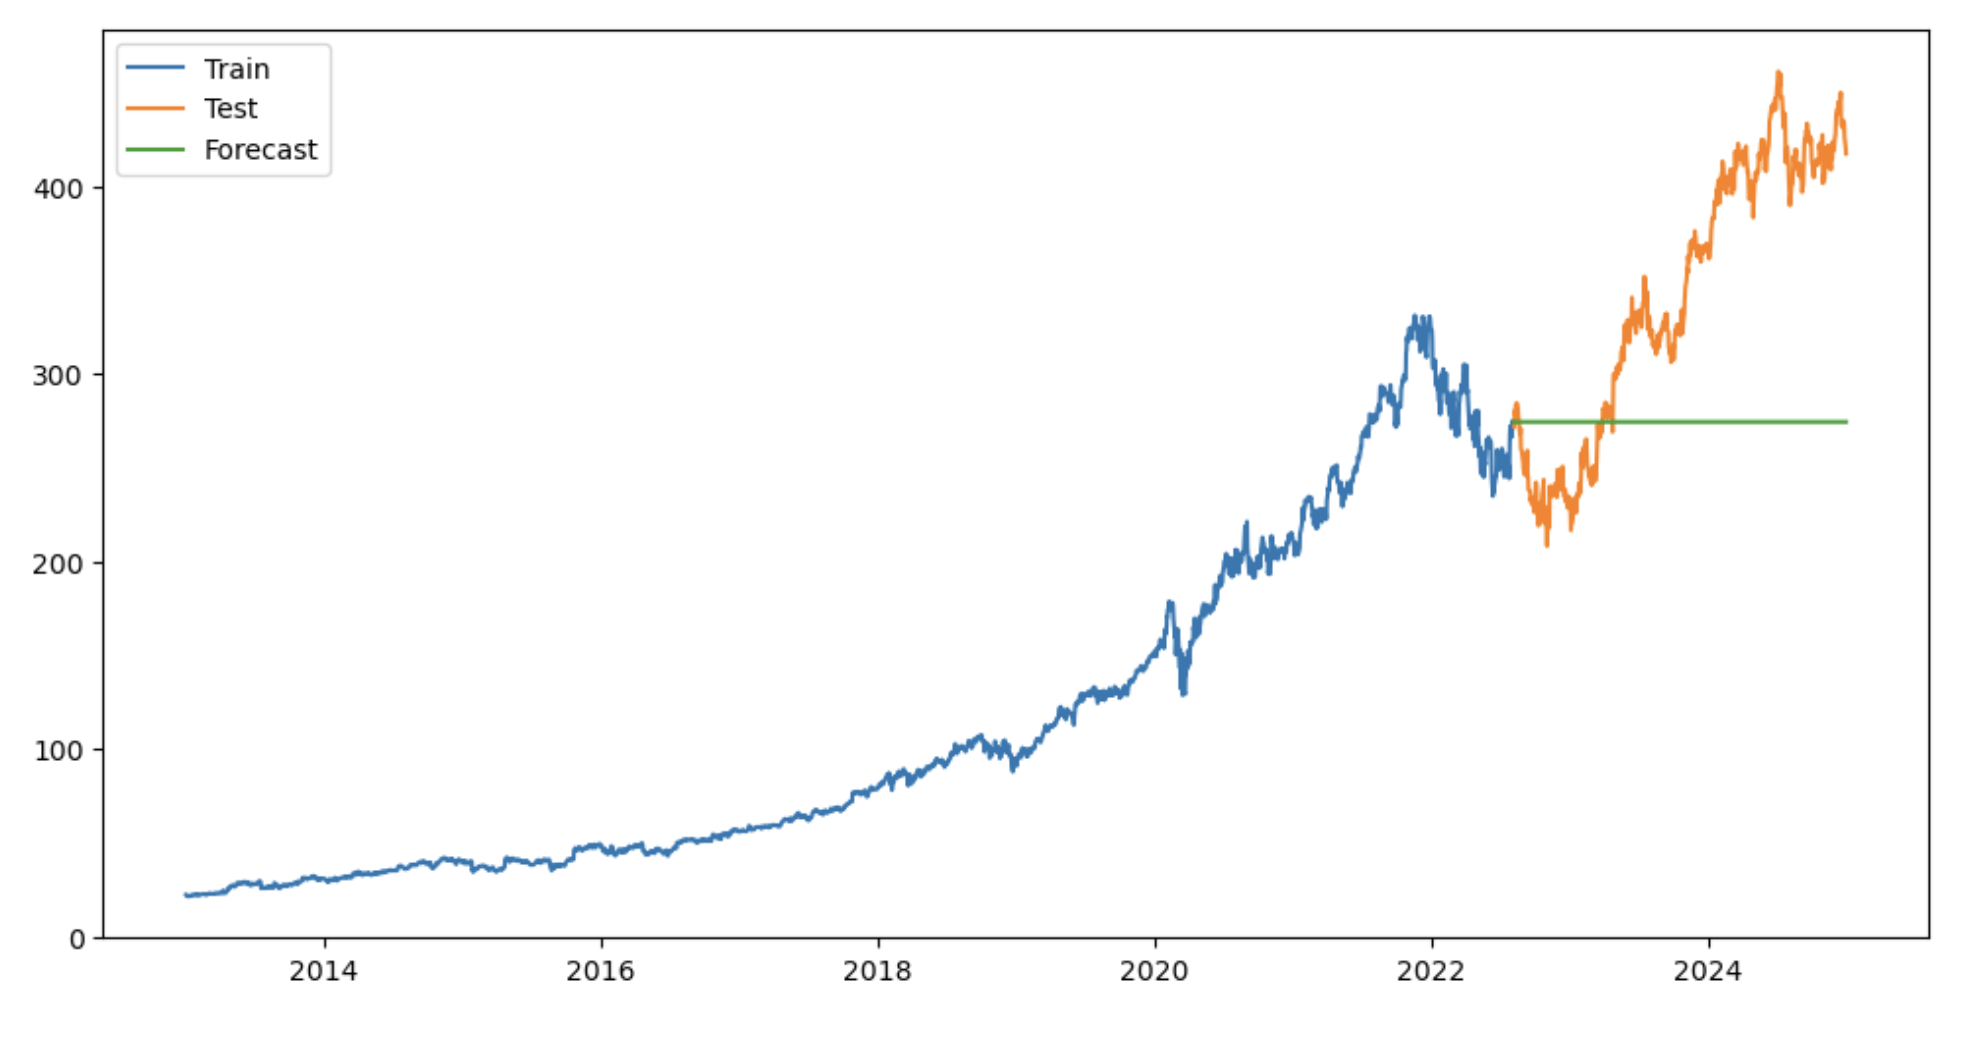
\includegraphics[width=0.95\textwidth]{LAB05/pics/step7_forecast.png}
    \caption{Kết quả dự báo ARIMA}
\end{figure}

\textbf{Nhận xét:}
\begin{itemize}
    \item Đường dự báo có xu hướng phẳng (flat)
    \item Không bắt được xu hướng tăng mạnh của dữ liệu thực tế
\end{itemize}

\textbf{Giải thích:}
\begin{itemize}
    \item Sai phân làm mất xu hướng dài hạn
    \item ARIMA chỉ học được phụ thuộc ngắn hạn
\end{itemize}

\subsection{Step 8: Đánh giá mô hình}

Tính các chỉ số đánh giá.

\begin{itemize}
    \item MAE: 83.19788165400618
    \item RMSE: 98.58069301407468
    \item MAPE: N/A
\end{itemize}

\textbf{Kết luận:}
\begin{itemize}
    \item Sai số còn tương đối lớn
    \item Mô hình chưa dự báo tốt
\end{itemize}

\subsection{Step 9: Tối ưu mô hình}

Sử dụng Grid Search để tìm mô hình tốt nhất.

\textbf{Kết quả:}
\begin{itemize}
    \item ARIMA(p,d,q) = (1,2,3)
    \item RMSE = 59.24645033427657
\end{itemize}
\begin{figure}[!htp]
    \centering
    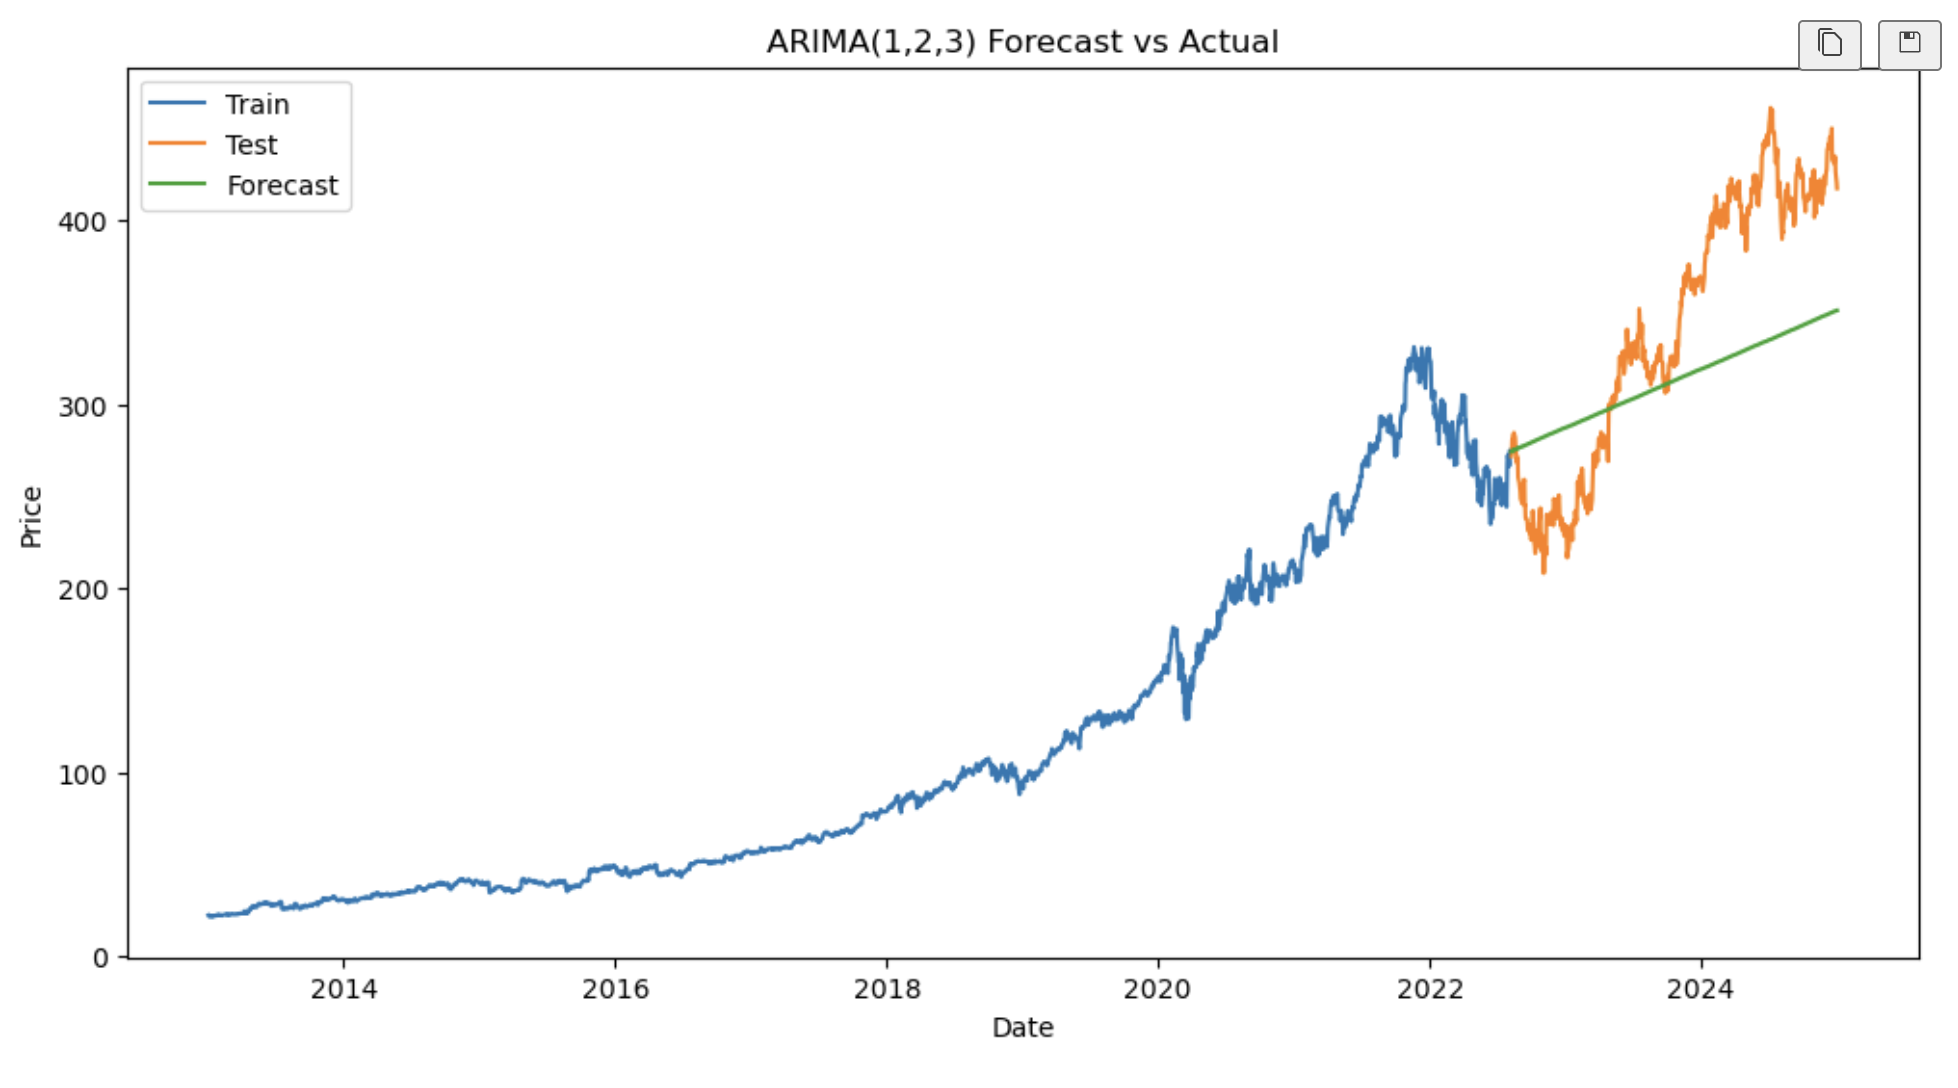
\includegraphics[width=0.95\textwidth]{LAB05/pics/step8.png}
    \caption{Kết quả dự báo ARIMA}
\end{figure}

\textbf{So sánh:}
\begin{itemize}
    \item Mô hình tối ưu có sai số thấp hơn
    \item Dự báo bám sát xu hướng tốt hơn
\end{itemize}

\textbf{Nhận xét:}
\begin{itemize}
    \item Mô hình cải thiện đáng kể so với ban đầu
    \item Tuy nhiên vẫn chưa capture tốt volatility
\end{itemize}

\subsection{Kết luận chung}

\begin{itemize}
    \item ARIMA là mô hình phù hợp để dự báo chuỗi thời gian cơ bản
    \item Tuy nhiên với dữ liệu tài chính:
    \begin{itemize}
        \item Biến động mạnh
        \item Phụ thuộc yếu tố bên ngoài
    \end{itemize}
    \item Cần sử dụng mô hình nâng cao như ARIMAX hoặc Machine Learning để cải thiện
\end{itemize}


\newpage
\section{Thực hiện bằng R}

\textbf{Dữ liệu được thu thập trực tiếp từ Yahoo Finance sử dụng thư viện \texttt{quantmod}.}

\subsection{Step 1: Thu thập dữ liệu}

Sử dụng hàm \texttt{getSymbols()} để lấy dữ liệu cổ phiếu MSFT từ năm 2013 đến 2025.

\begin{figure}[!htp]
    \centering
    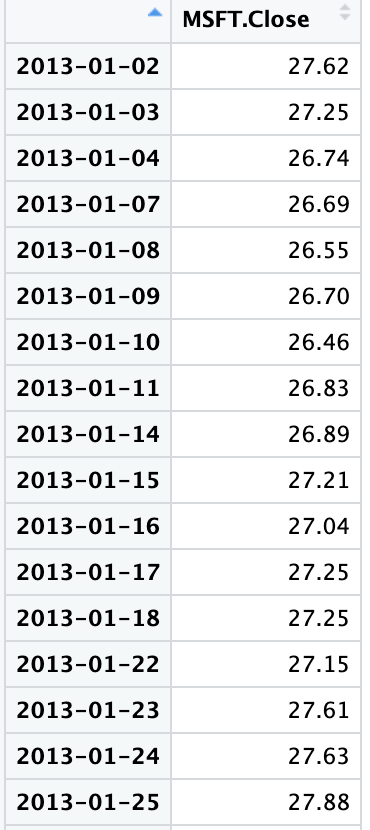
\includegraphics[width=0.4\textwidth]{LAB05/pics/r_step1_data.png}
    \caption{Dữ liệu MSFT từ Yahoo Finance}
\end{figure}

\subsection{Step 2: Trực quan hóa dữ liệu}

\begin{figure}[!htp]
    \centering
    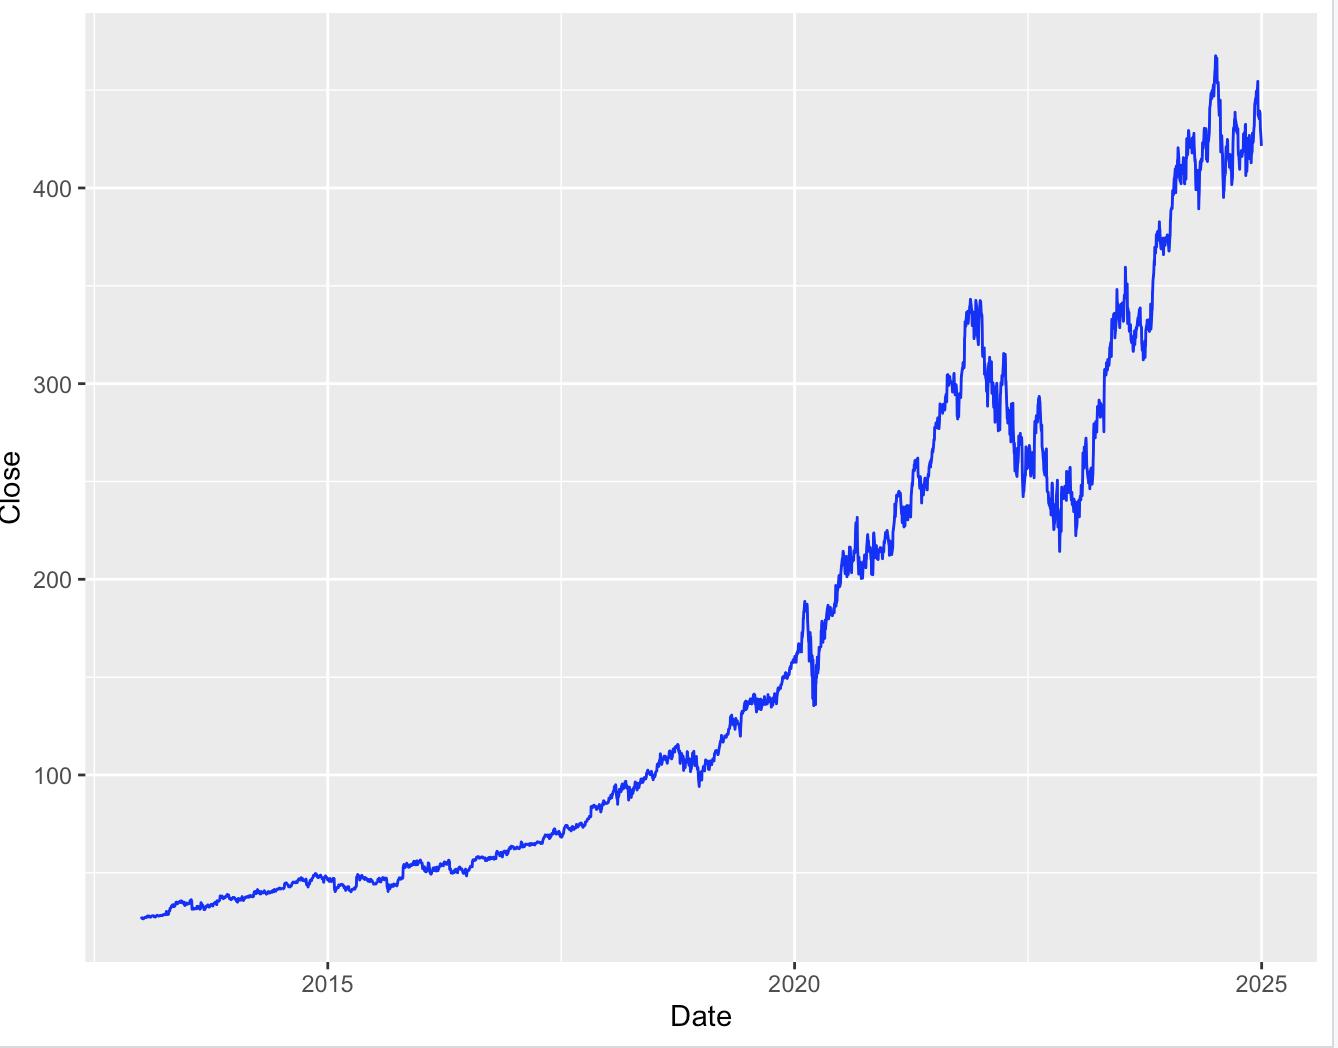
\includegraphics[width=0.95\textwidth]{LAB05/pics/r_step2_plot.png}
    \caption{Biểu đồ giá cổ phiếu MSFT}
\end{figure}

\textbf{Nhận xét:}
\begin{itemize}
    \item Dữ liệu có xu hướng tăng theo thời gian
    \item Chuỗi không dừng
\end{itemize}

\subsection{Step 3: Chuyển đổi chuỗi thời gian}

Chuyển dữ liệu về dạng time series với tần suất 252 (ngày giao dịch).

\subsection{Step 4: Kiểm định ADF}

Thực hiện kiểm định Augmented Dickey-Fuller.

\textbf{Kết luận:}
\begin{itemize}
    \item p-value > 0.05 $\Rightarrow$ chuỗi không dừng
\end{itemize}

\subsection{Step 5: Sai phân}

Thực hiện sai phân bậc 1.

\begin{figure}[!htp]
    \centering
    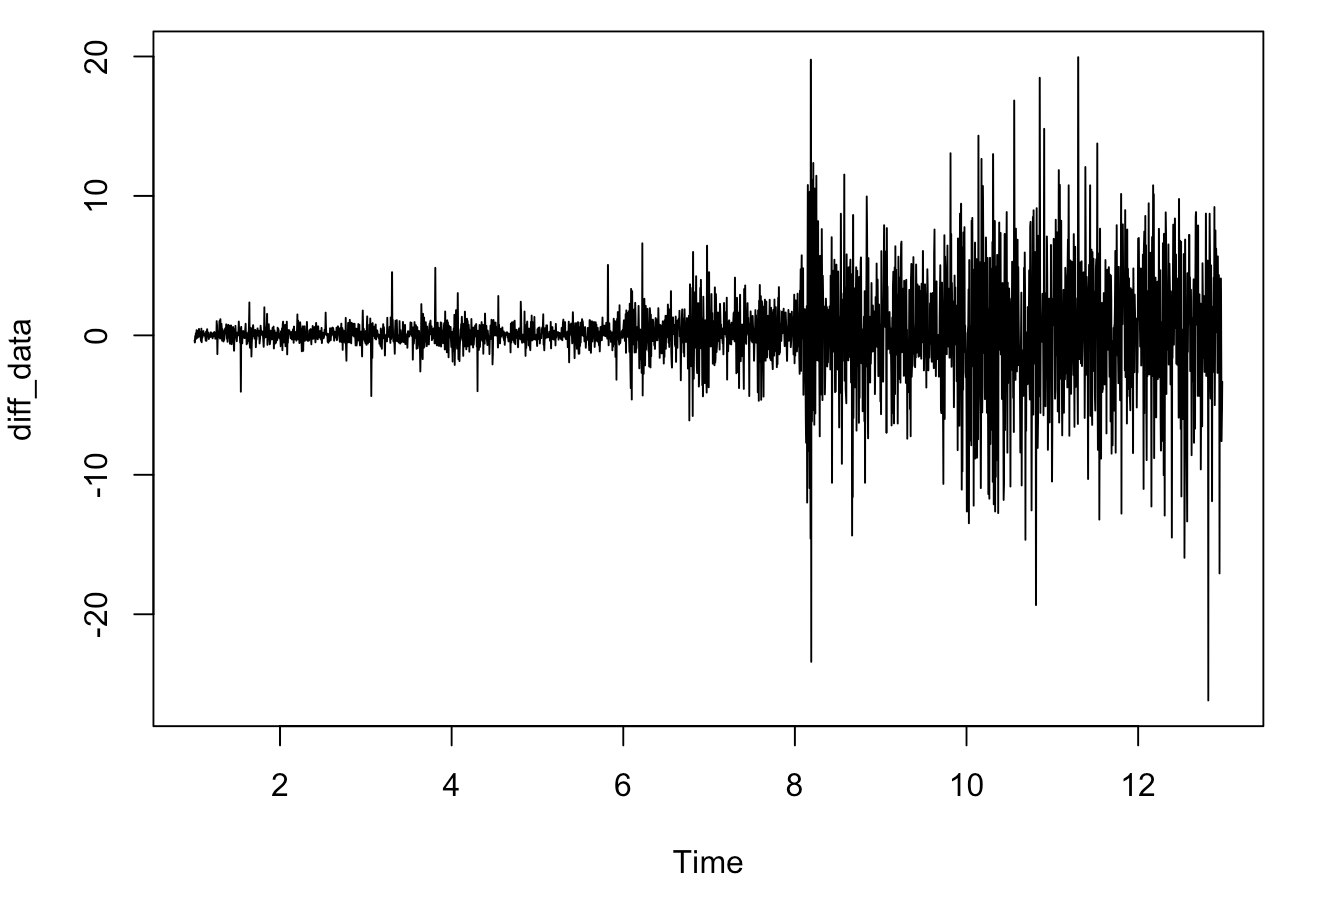
\includegraphics[width=0.95\textwidth]{LAB05/pics/r_step5_diff.png}
    \caption{Chuỗi sau khi sai phân}
\end{figure}

\textbf{Kết luận:}
\begin{itemize}
    \item p-value < 0.05 $\Rightarrow$ chuỗi dừng
    \item Chọn $d = 1$
\end{itemize}

\subsection{Step 6: ACF và PACF}

\begin{figure}[!htp]
    \centering
    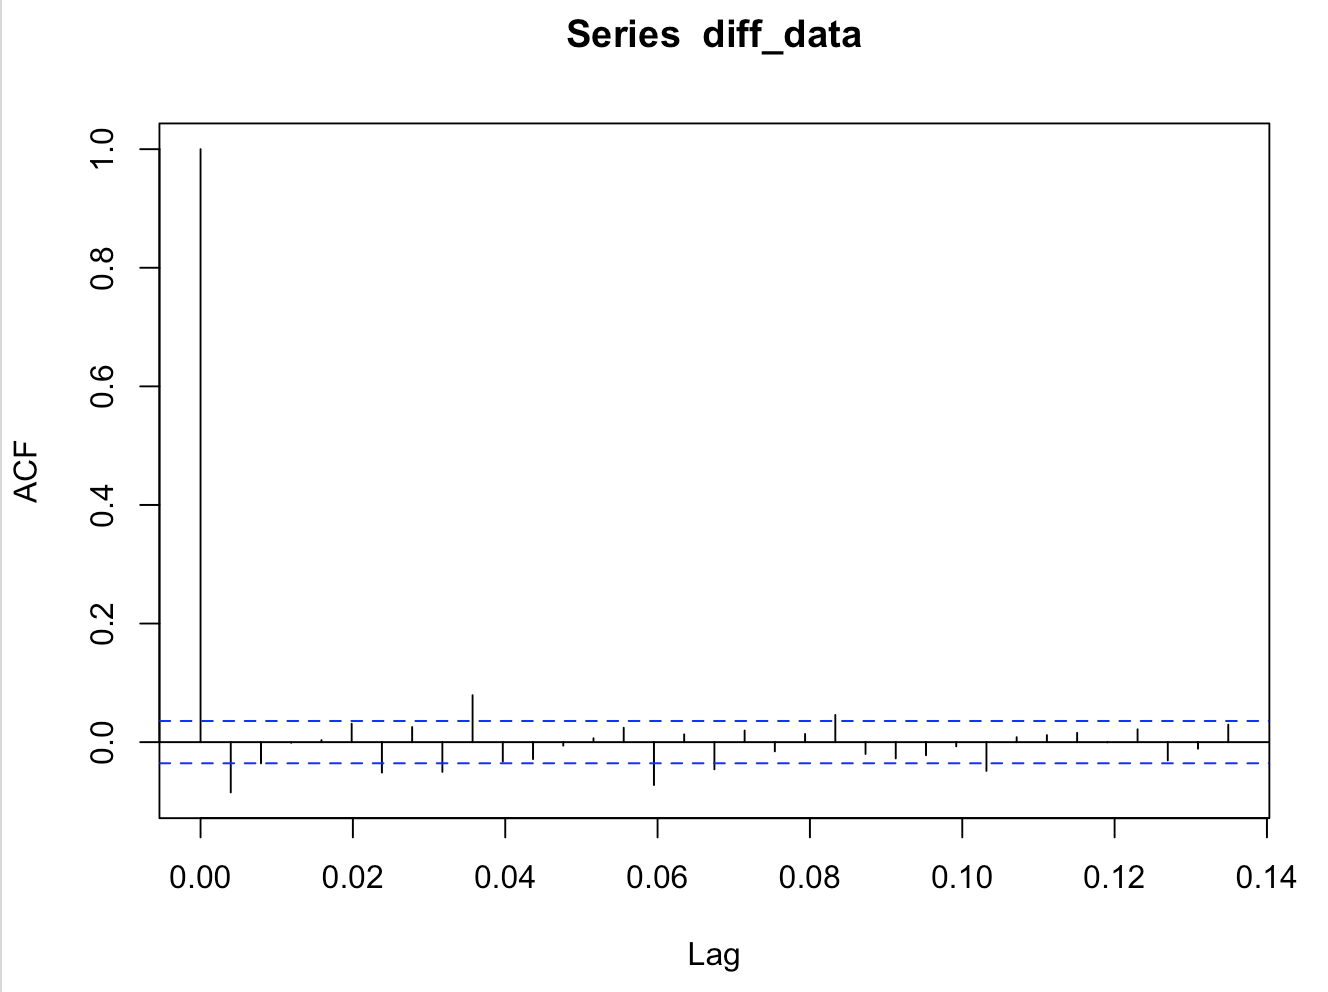
\includegraphics[width=0.95\textwidth]{LAB05/pics/r_step6_acf.png}
    \caption{Biểu đồ ACF}
\end{figure}

\begin{figure}[!htp]
    \centering
    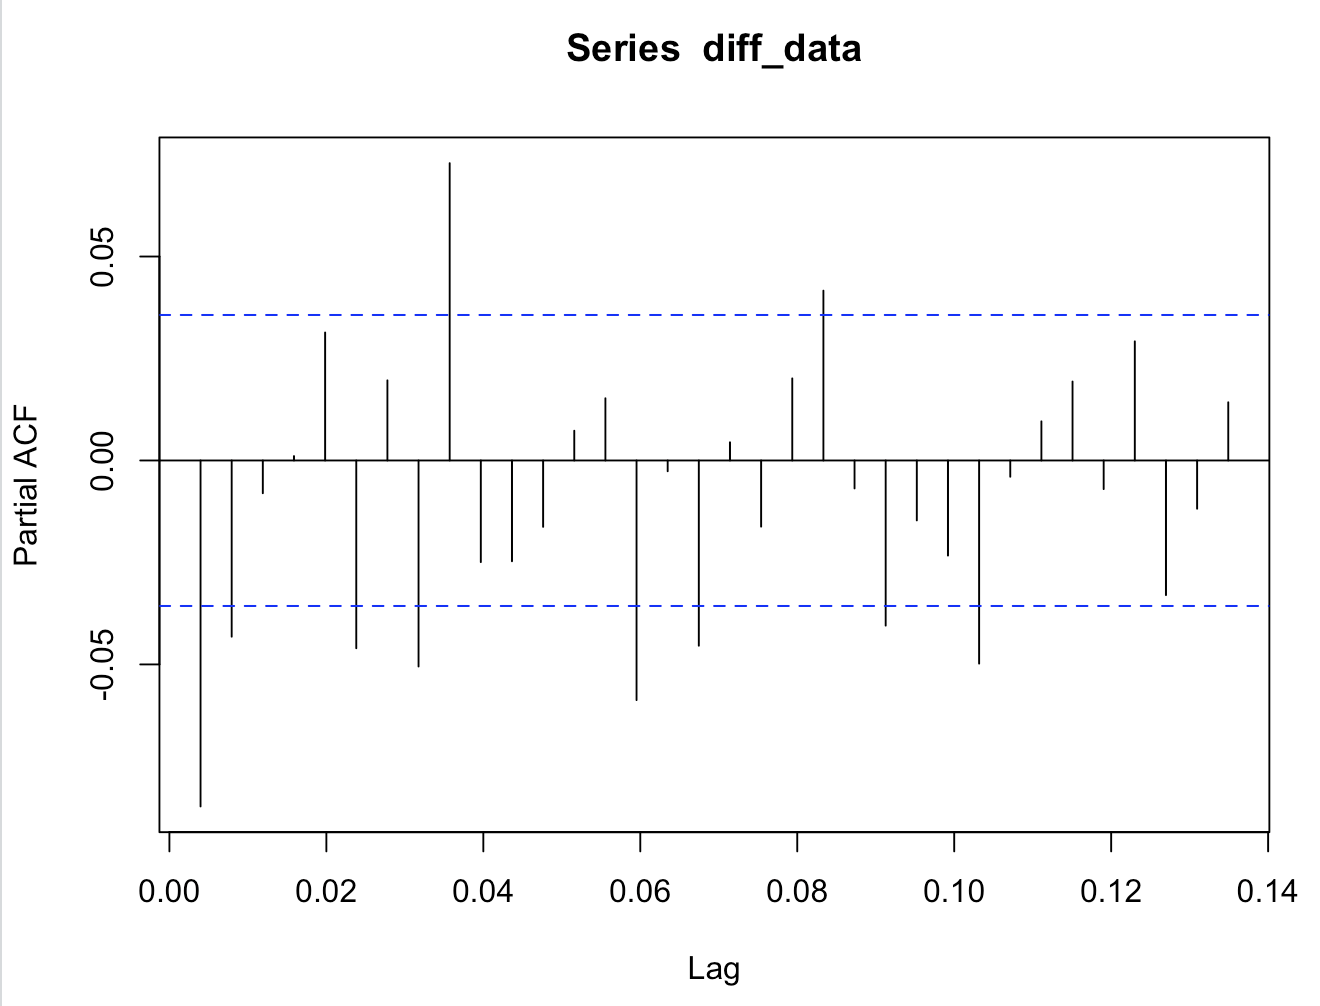
\includegraphics[width=0.95\textwidth]{LAB05/pics/r_step6_pacf.png}
    \caption{Biểu đồ PACF}
\end{figure}

\textbf{Kết luận:}
\begin{itemize}
    \item Chọn $p = 1$
    \item Chọn $q = 1$
\end{itemize}

$\Rightarrow$ Mô hình ban đầu: \textbf{ARIMA(1,1,1)}

\subsection{Step 7: Xây dựng mô hình}

Xây dựng mô hình ARIMA trên tập train.

\subsection{Step 8: Dự báo}

\begin{figure}[!htp]
    \centering
    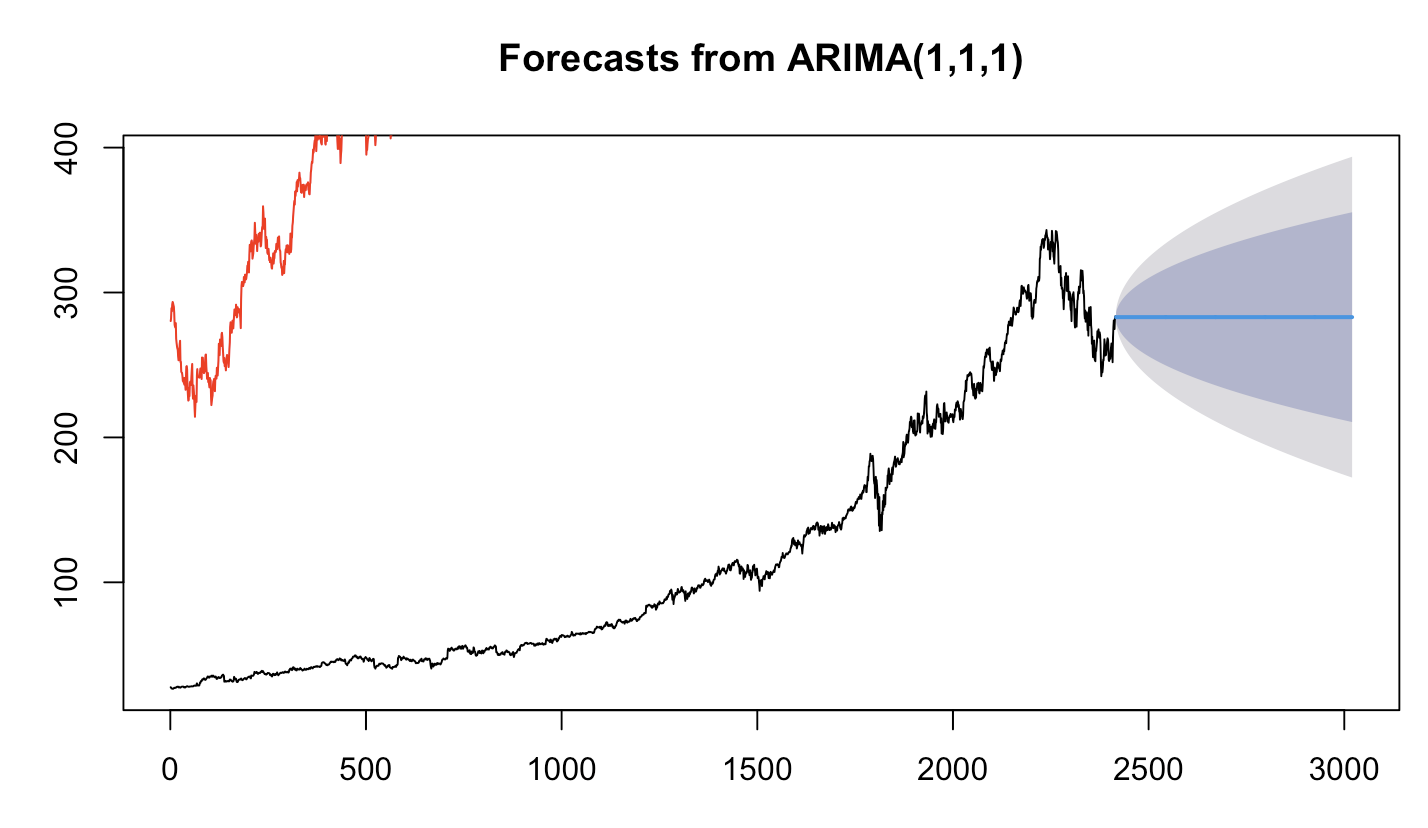
\includegraphics[width=0.95\textwidth]{LAB05/pics/r_step8_forecast.png}
    \caption{Kết quả dự báo ARIMA}
\end{figure}

\textbf{Nhận xét:}
\begin{itemize}
    \item Đường dự báo có xu hướng phẳng
    \item Chưa bám sát dữ liệu thực tế
\end{itemize}

\subsection{Step 9: Đánh giá mô hình}

Các chỉ số:
\begin{itemize}
    \item RMSE: 96.63541
    \item MAE: 81.85936
    \item MAPE: 21.80617
\end{itemize}

\subsection{Step 10: Auto ARIMA}

Áp dụng hàm \texttt{auto.arima()} để tìm mô hình tối ưu.

\begin{figure}[!htp]
    \centering
    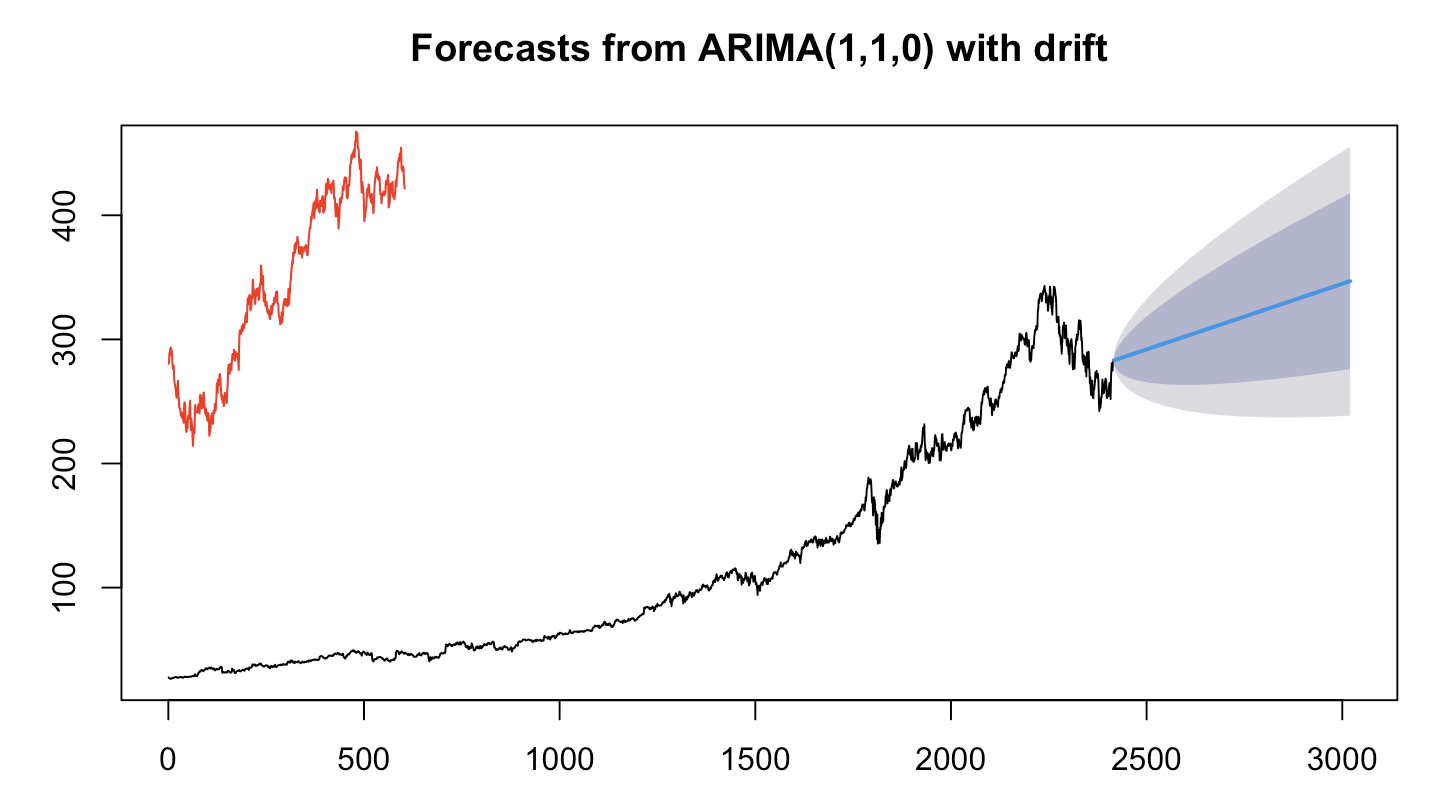
\includegraphics[width=0.95\textwidth]{LAB05/pics/r_step10_auto.png}
    \caption{Dự báo bằng Auto ARIMA}
\end{figure}

\textbf{Kết luận:}
\begin{itemize}
    \item Auto ARIMA cho kết quả tốt hơn
    \item Sai số giảm so với mô hình ban đầu
\end{itemize}

\subsection{Kết luận chung}

\begin{itemize}
    \item ARIMA phù hợp để mô hình hóa chuỗi thời gian
    \item Tuy nhiên chưa capture tốt volatility
    \item Cần mô hình nâng cao như ARIMAX để cải thiện
\end{itemize}

\newpage
\section{Thực hiện phân tích chuỗi thời gian bằng SPSS}

\subsection{Step 2: Biểu đồ chuỗi thời gian}

Dữ liệu giá đóng cửa cổ phiếu MSFT được nhập vào SPSS và thiết lập dưới dạng chuỗi thời gian bằng cách xác định biến thời gian (Date). Biểu đồ chuỗi thời gian được vẽ nhằm quan sát xu hướng và đặc điểm của dữ liệu.

\begin{figure}[!htp]
    \centering
    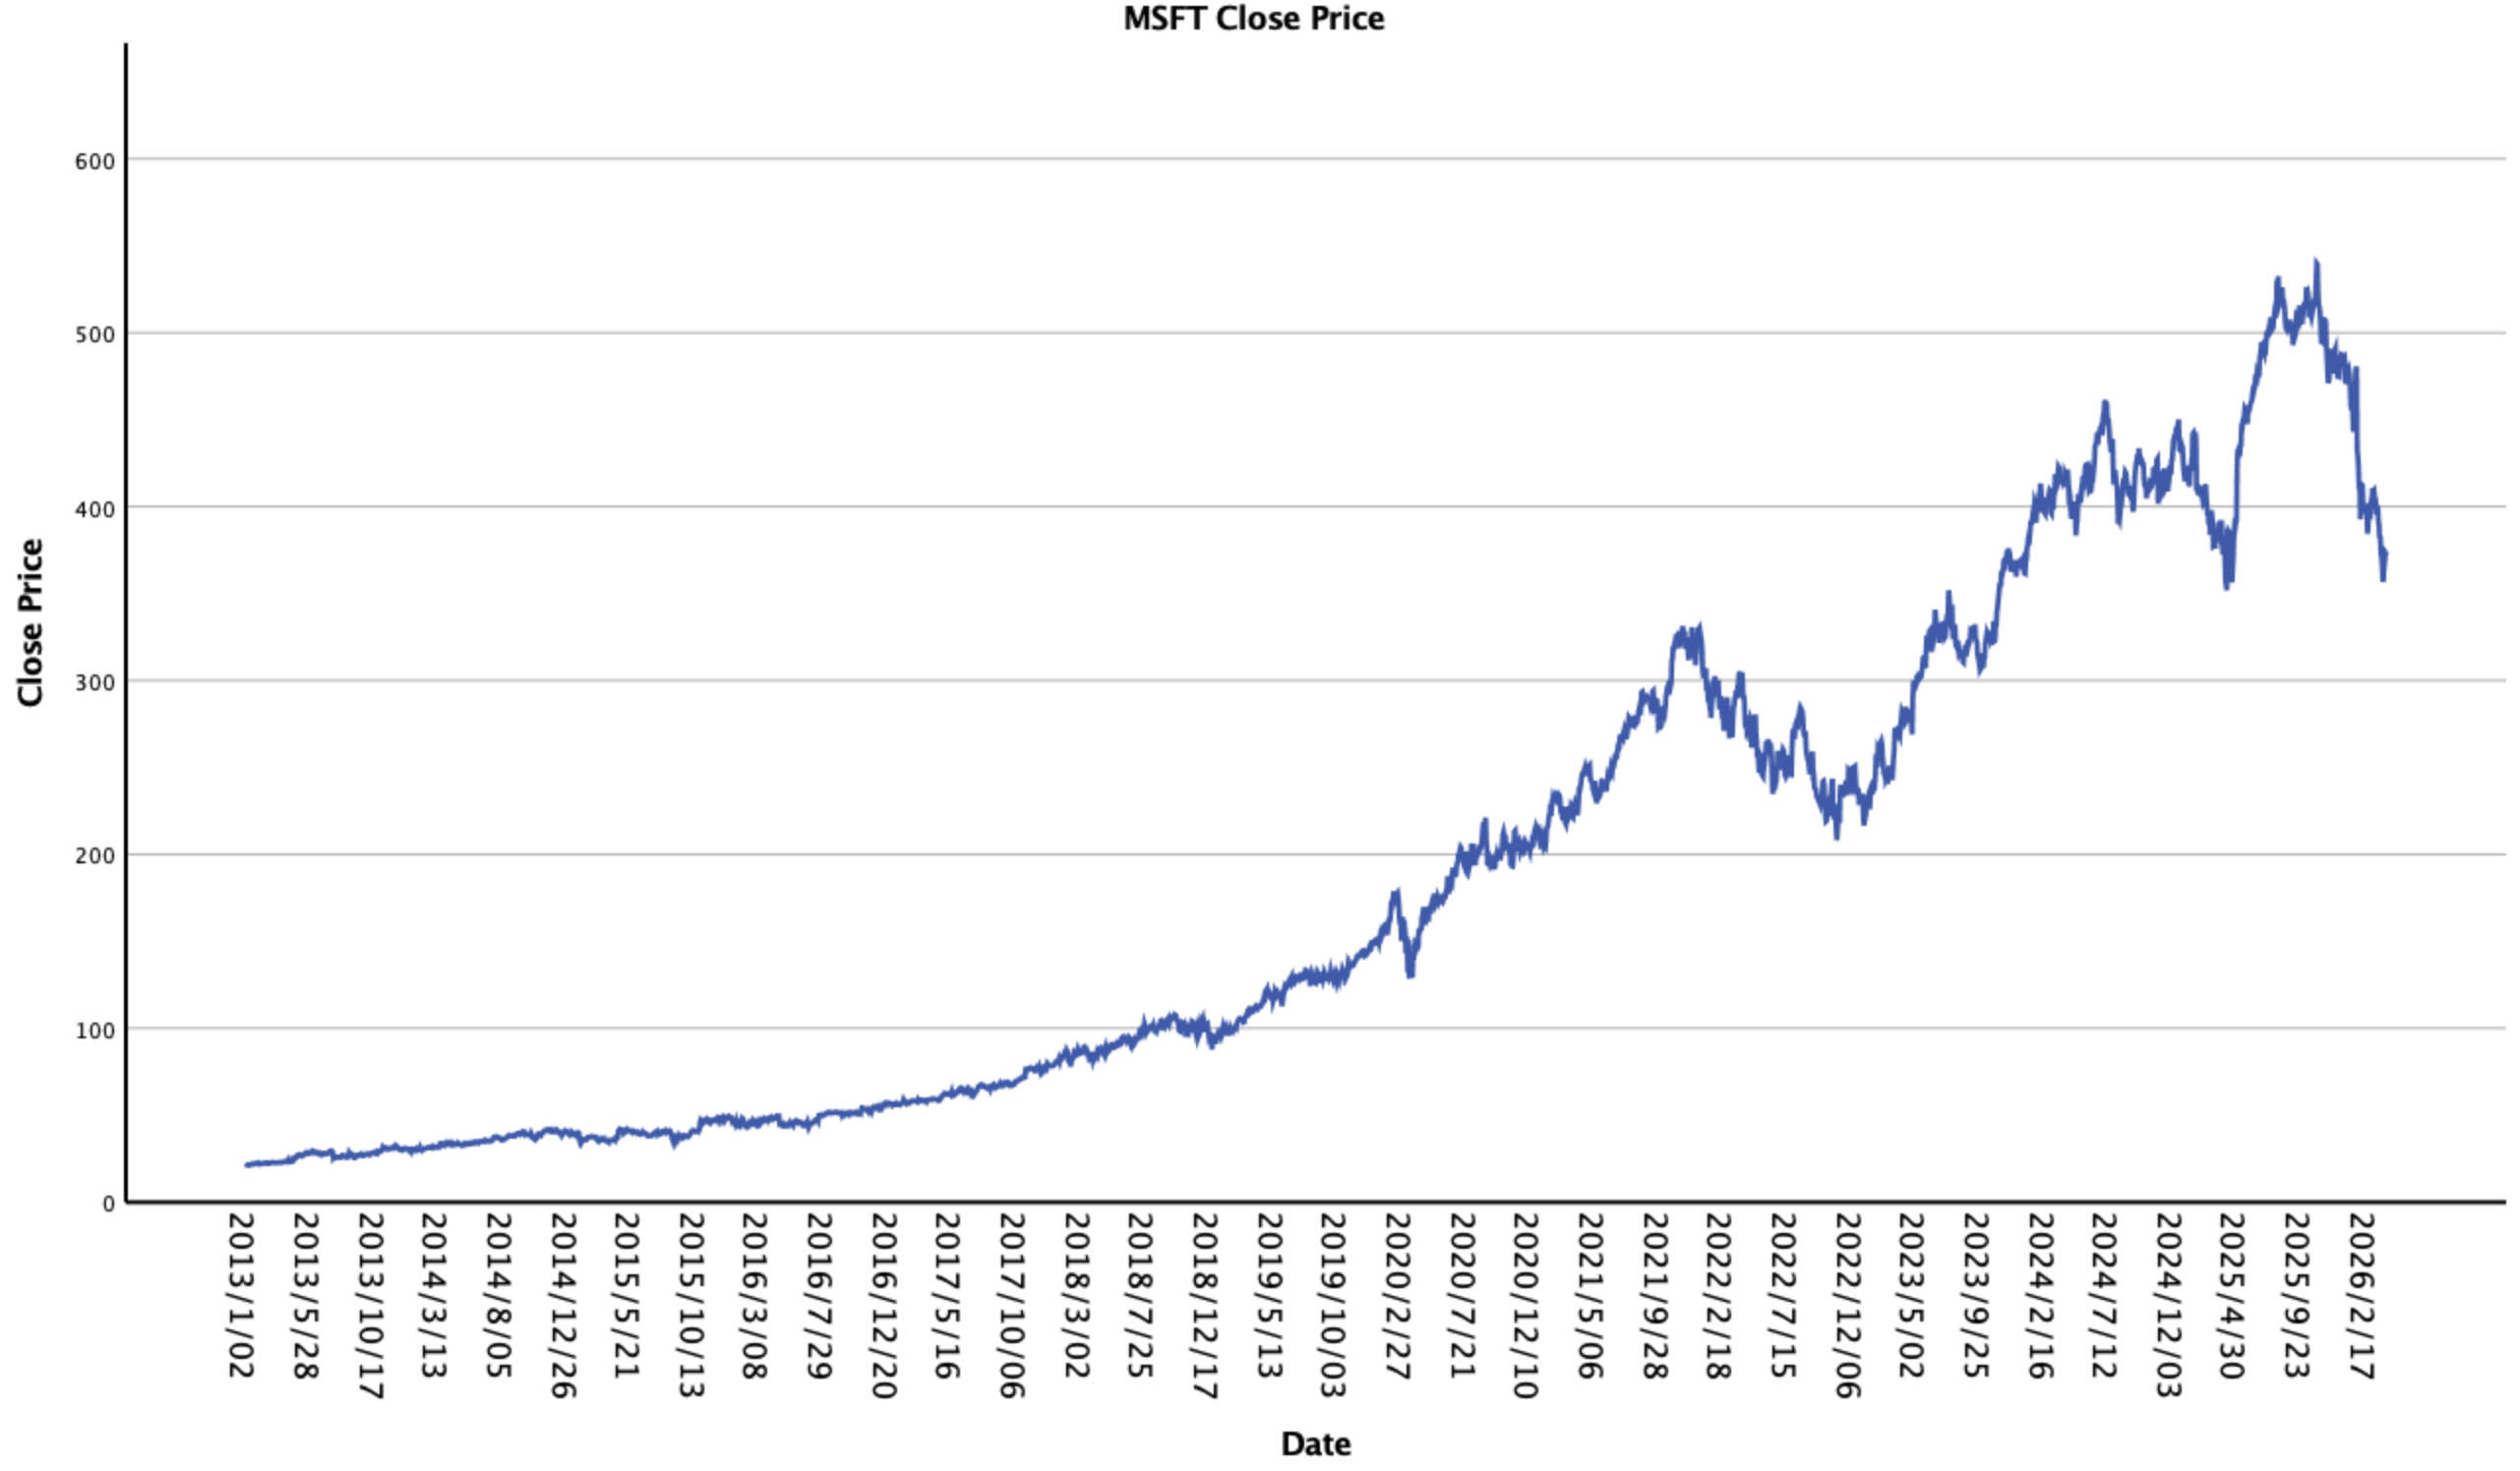
\includegraphics[width=0.95\textwidth]{LAB05/pics/plot_timeseries.png}
    \caption{Biểu đồ chuỗi thời gian giá đóng cửa MSFT}
\end{figure}

Biểu đồ cho thấy dữ liệu có xu hướng tăng rõ rệt theo thời gian, do đó chuỗi ban đầu không có tính dừng.

\subsection{Step 3: Kiểm tra tính dừng}

Do chuỗi có xu hướng, tiến hành lấy sai phân bậc 1 để làm dừng dữ liệu.

\begin{figure}[!htp]
    \centering
    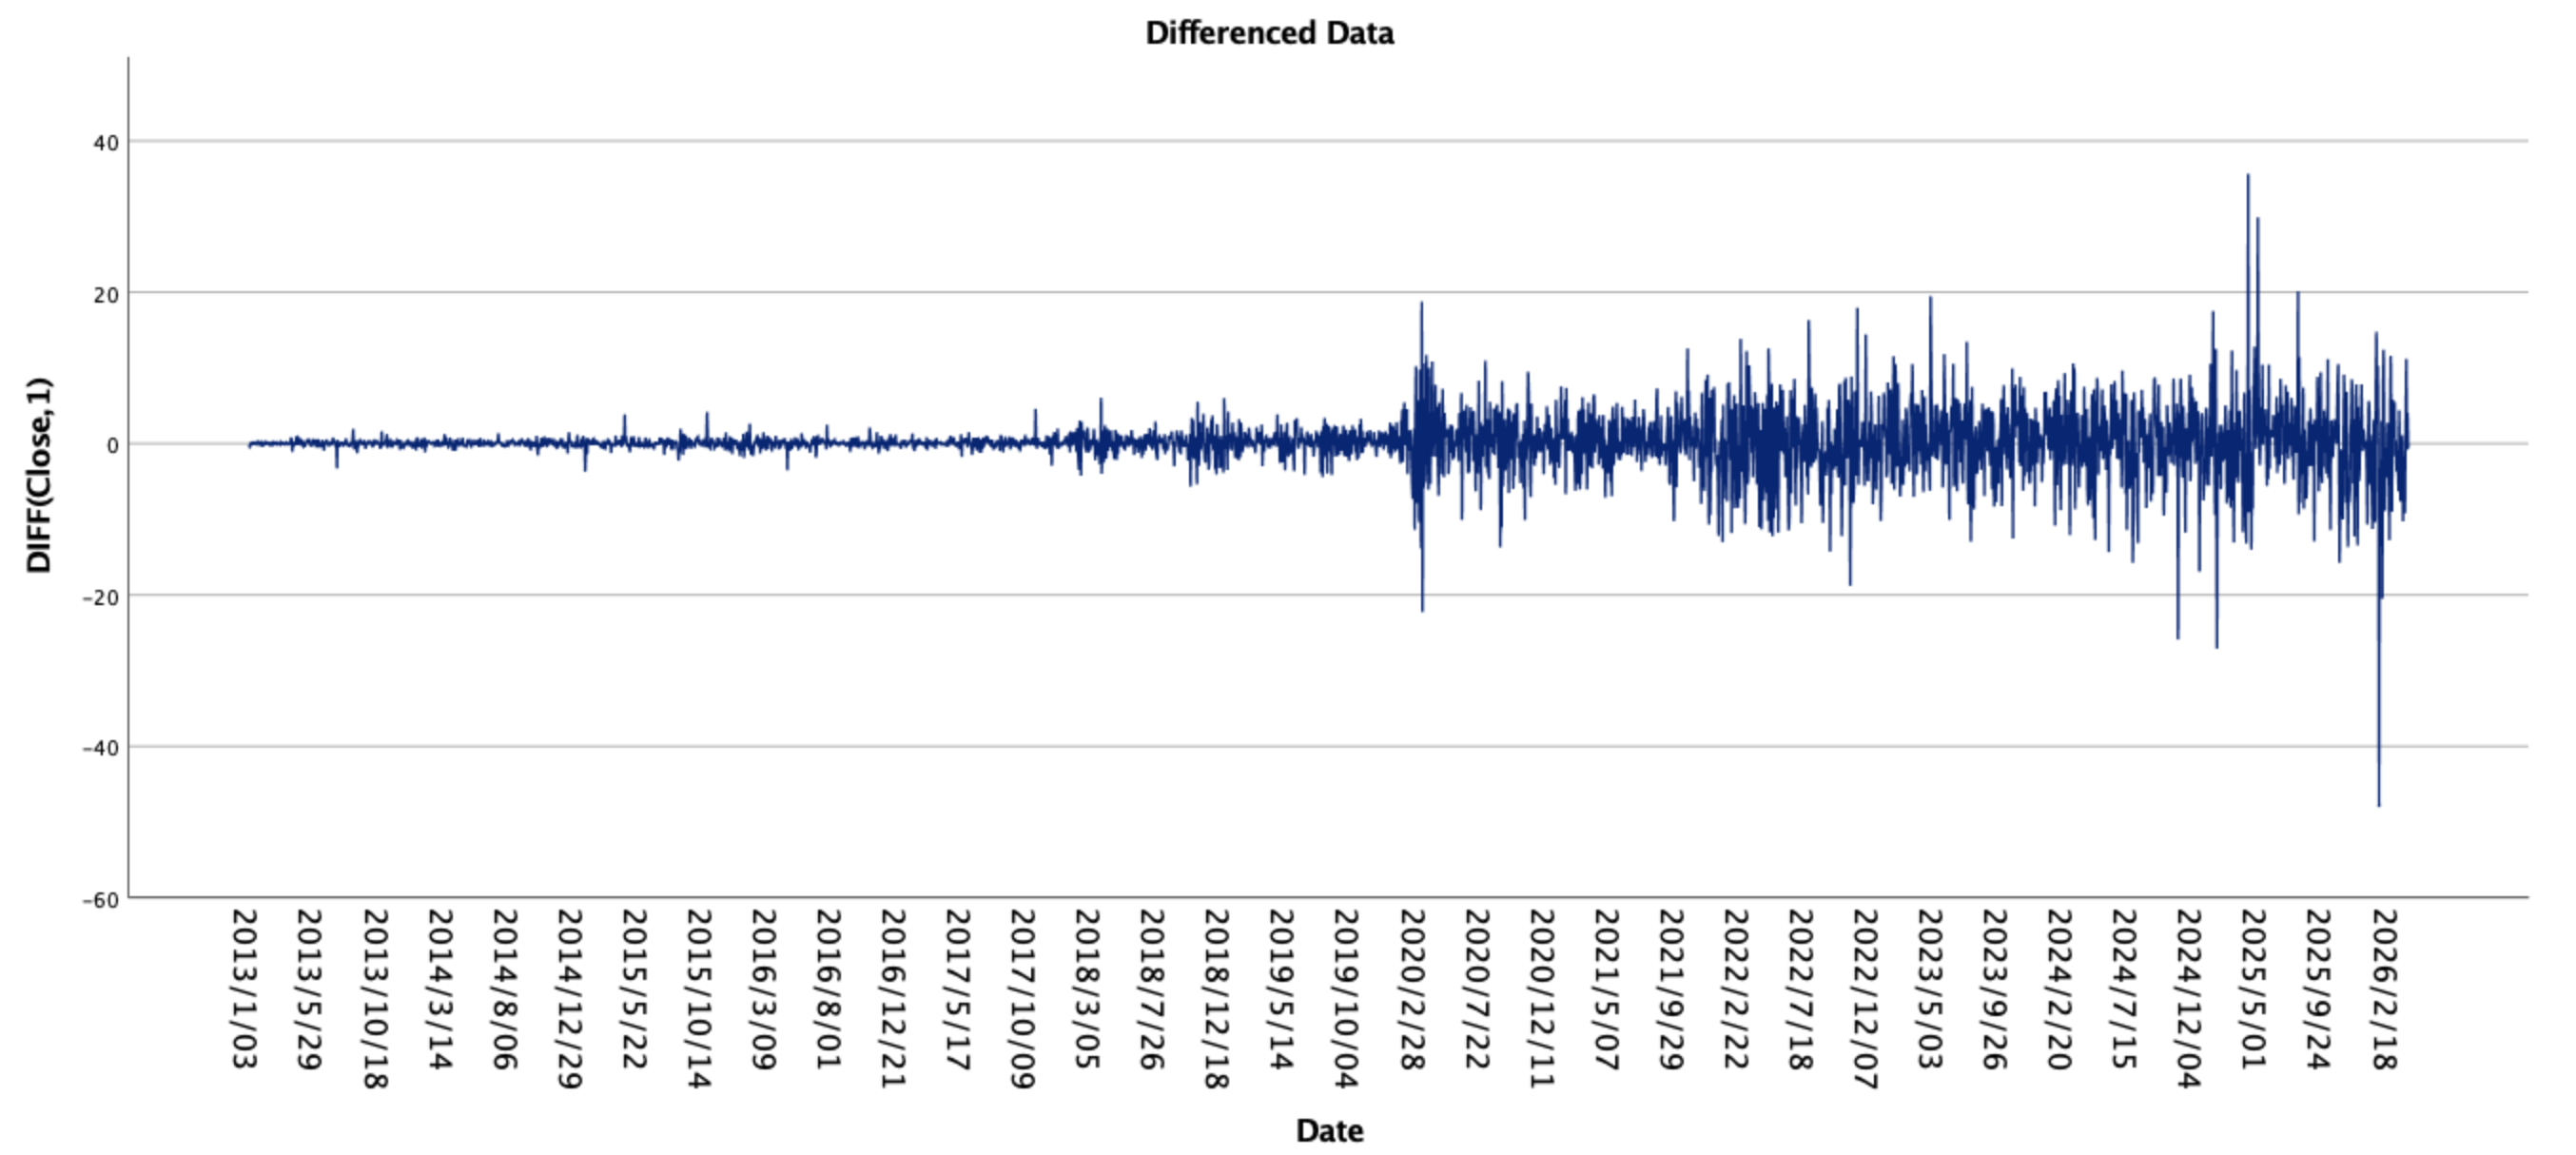
\includegraphics[width=0.95\textwidth]{LAB05/pics/differenced_series.png}
    \caption{Chuỗi sau khi sai phân bậc 1}
\end{figure}

Sau khi thực hiện sai phân, chuỗi dao động quanh giá trị trung bình ổn định hơn, cho thấy chuỗi đã trở nên dừng và phù hợp để xây dựng mô hình ARIMA.

\subsection{Step 4: Xác định tham số p và q}

Biểu đồ ACF và PACF được sử dụng để xác định các tham số của mô hình ARIMA.

\begin{figure}[!htp]
    \centering
    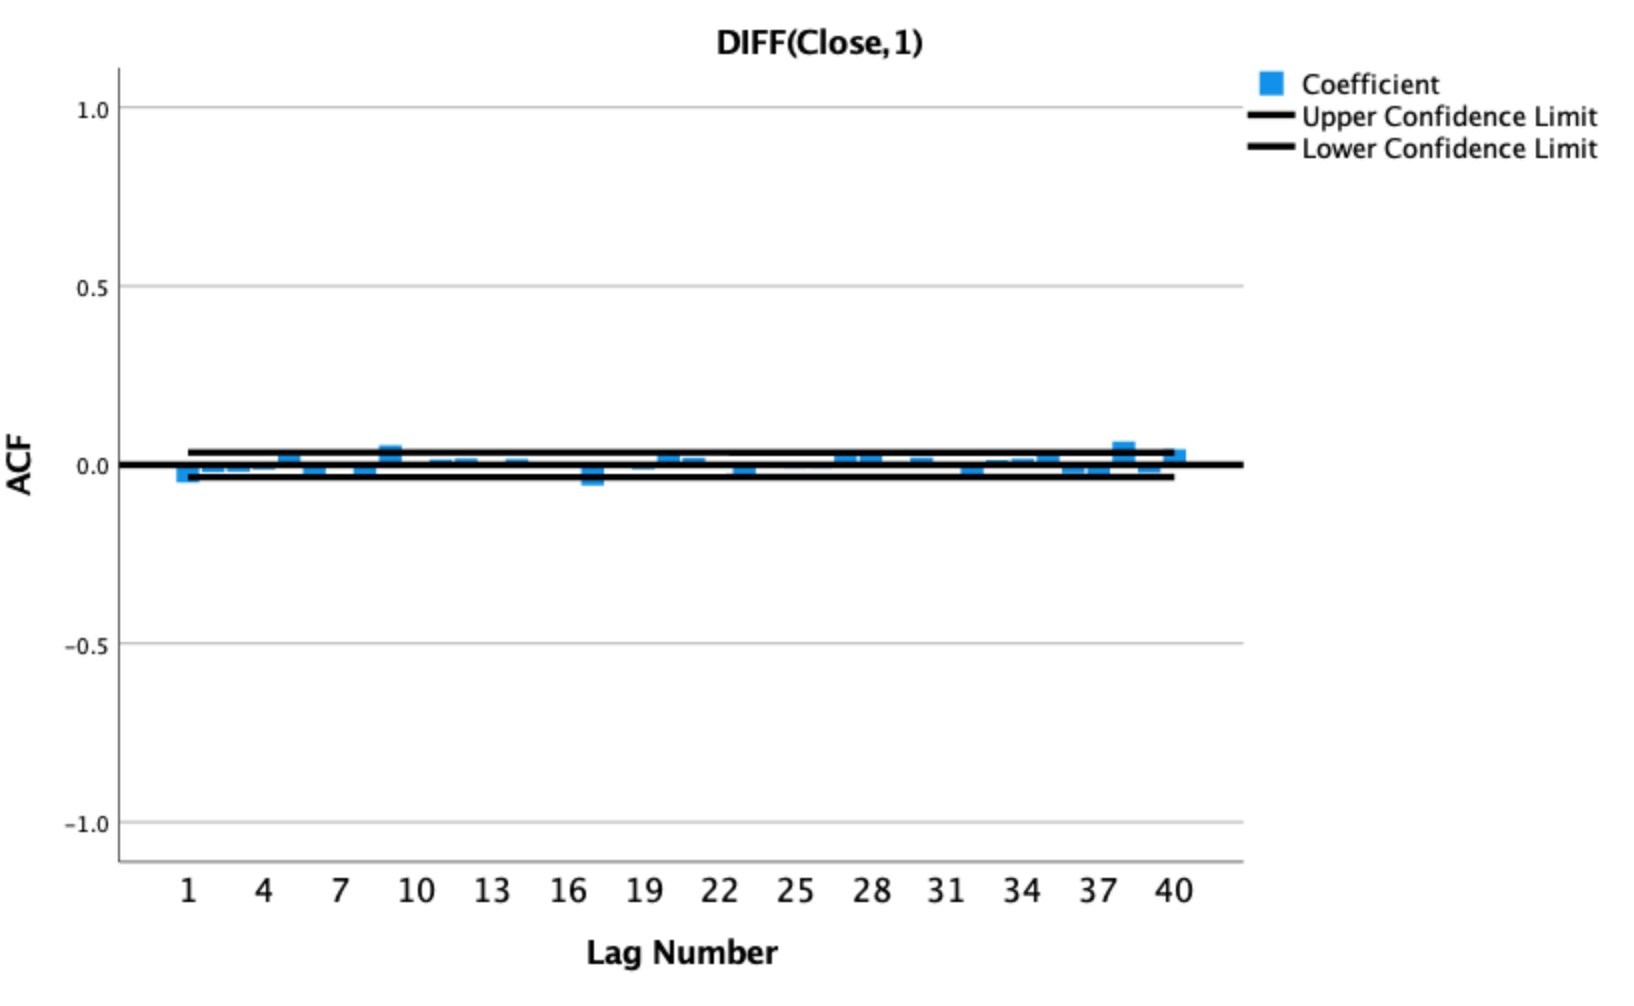
\includegraphics[width=0.95\textwidth]{LAB05/pics/acf.png}
    \caption{Biểu đồ ACF}
\end{figure}

Kết quả cho thấy các hệ số tự tương quan đều nằm trong khoảng tin cậy và không có lag nào có ý nghĩa thống kê. Do đó, không cần thành phần MA (q = 0).

Tương tự, PACF không cho thấy sự cắt cụt rõ ràng, do đó không cần thành phần AR (p = 0).

Vì vậy, mô hình được đề xuất là ARIMA(0,1,0).

\subsection{Step 5: Xây dựng mô hình ARIMA}

Mô hình ARIMA(0,1,0) được xây dựng trong SPSS.

\begin{figure}[!htp]
    \centering
    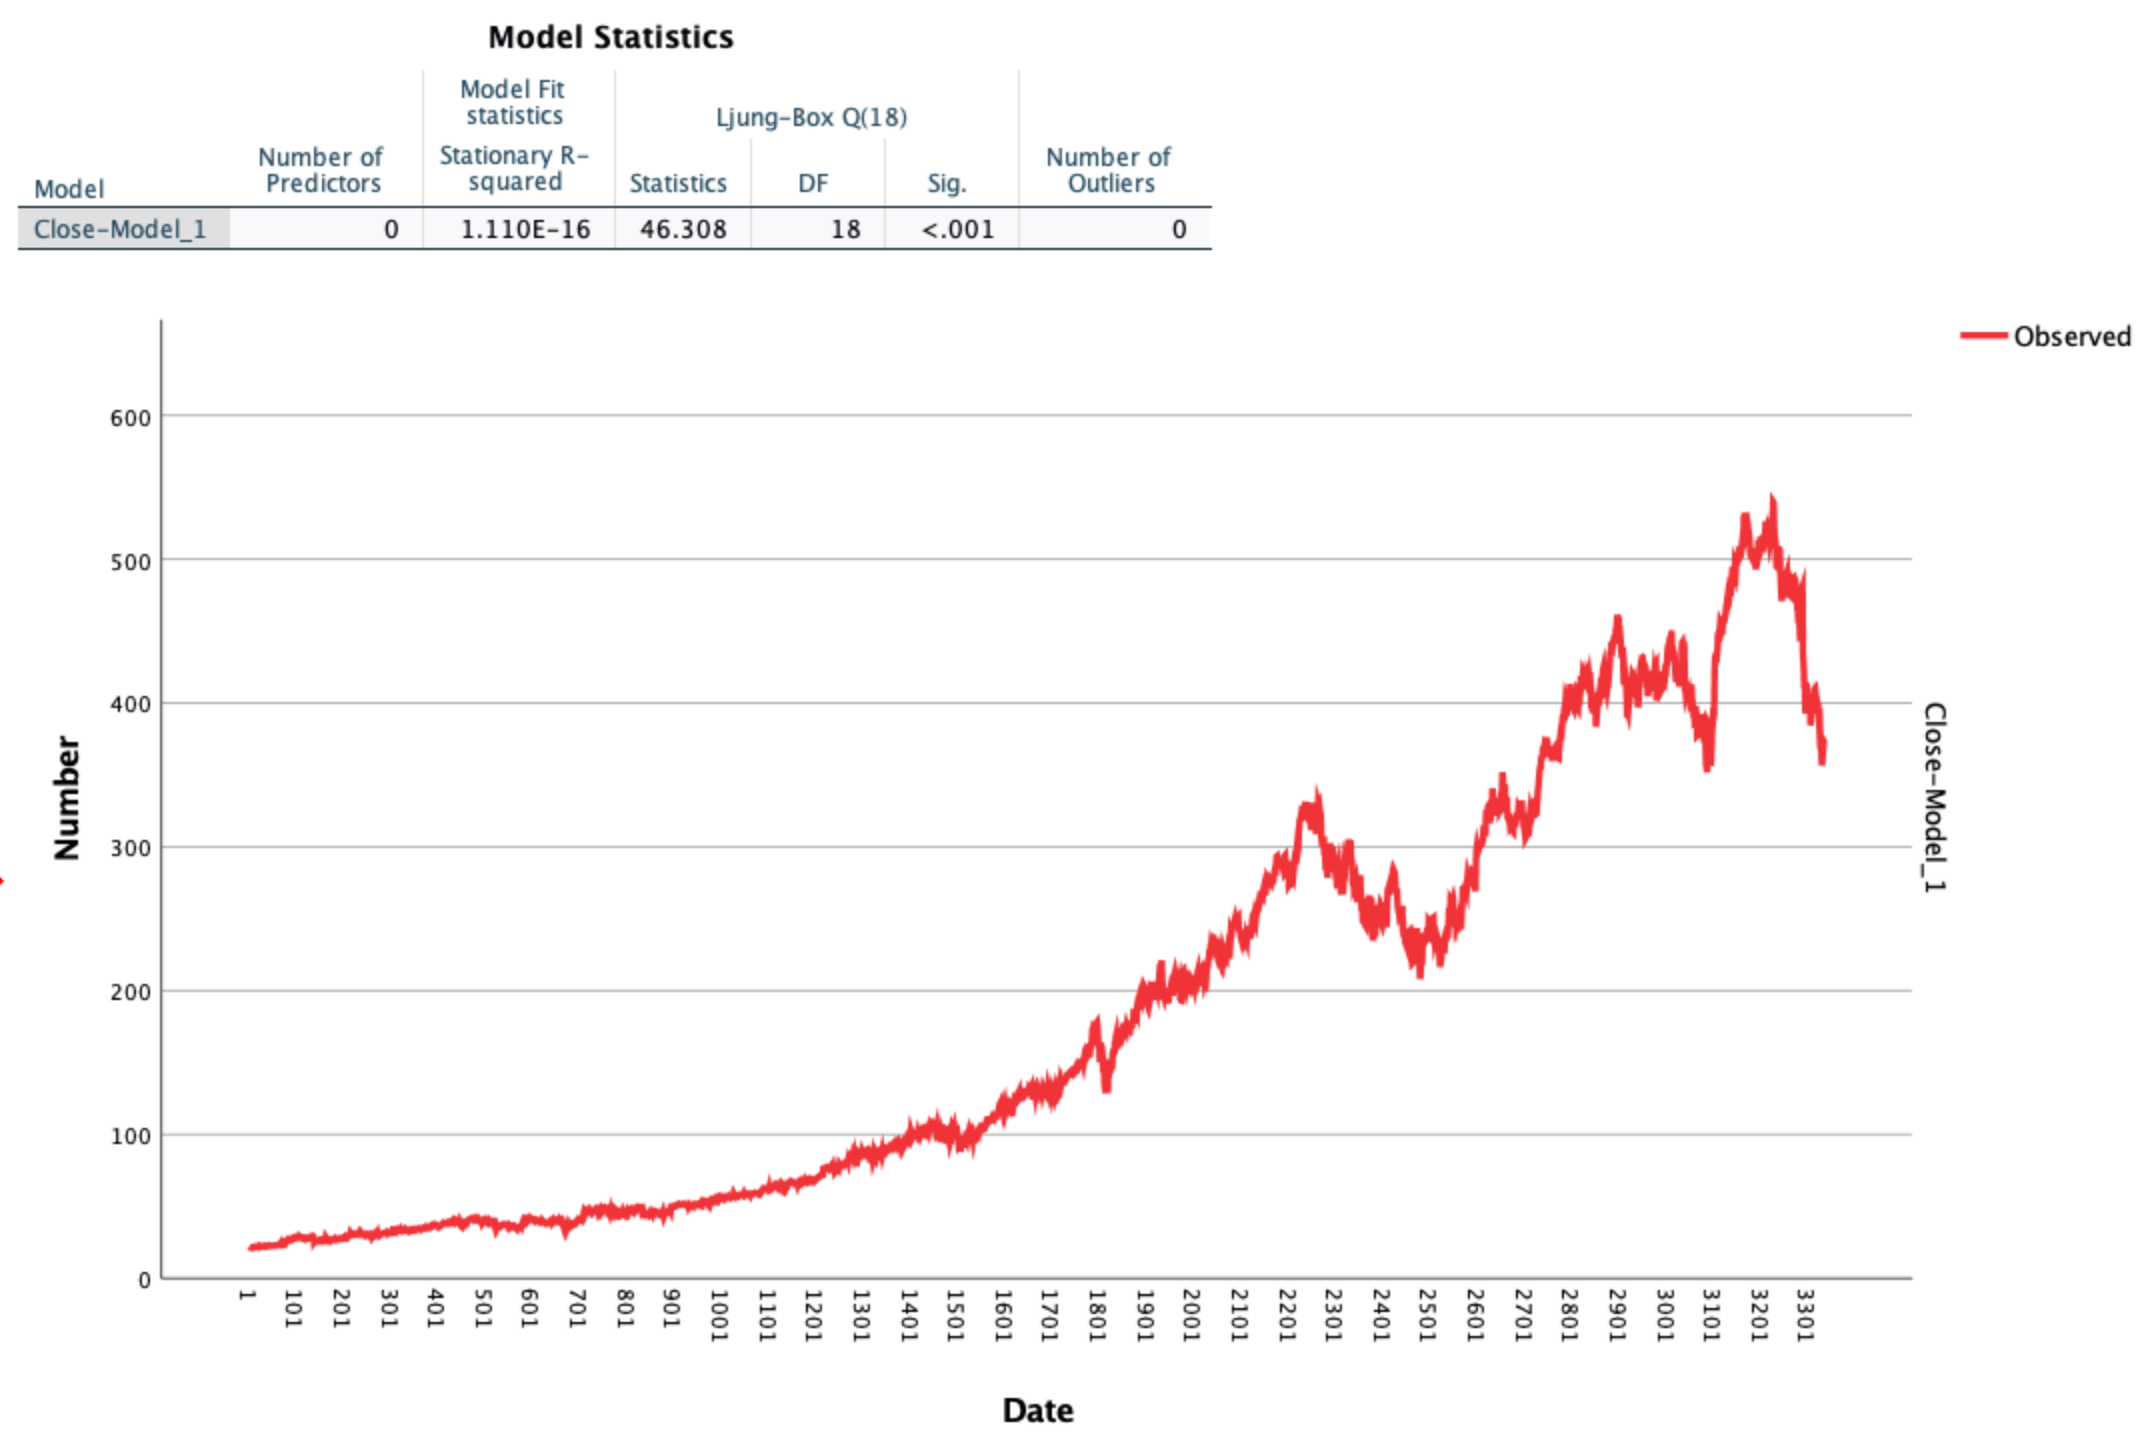
\includegraphics[width=0.95\textwidth]{LAB05/pics/arima_model.png}
    \caption{Kết quả mô hình ARIMA(0,1,0)}
\end{figure}

Mô hình không bao gồm thành phần AR và MA, cho thấy chuỗi sau sai phân không còn tự tương quan đáng kể.

\subsection{Step 6: Đánh giá mô hình}

Các chỉ số đánh giá mô hình:

\begin{itemize}
    \item RMSE = 3.731
    \item MAE = 2.125
    \item MAPE = 1.142\%
\end{itemize}

Các chỉ số này cho thấy sai số dự báo ở mức thấp và mô hình có độ chính xác cao.

Tuy nhiên, kiểm định Ljung-Box cho p-value < 0.05 cho thấy phần dư vẫn còn tự tương quan, chứng tỏ mô hình chưa hoàn toàn phù hợp.

\subsection{Step 8: Lựa chọn mô hình tối ưu bằng Expert Modeler}

Sử dụng chức năng Expert Modeler trong SPSS, mô hình tối ưu được lựa chọn là ARIMA(2,1,8).

\begin{figure}[!htp]
    \centering
    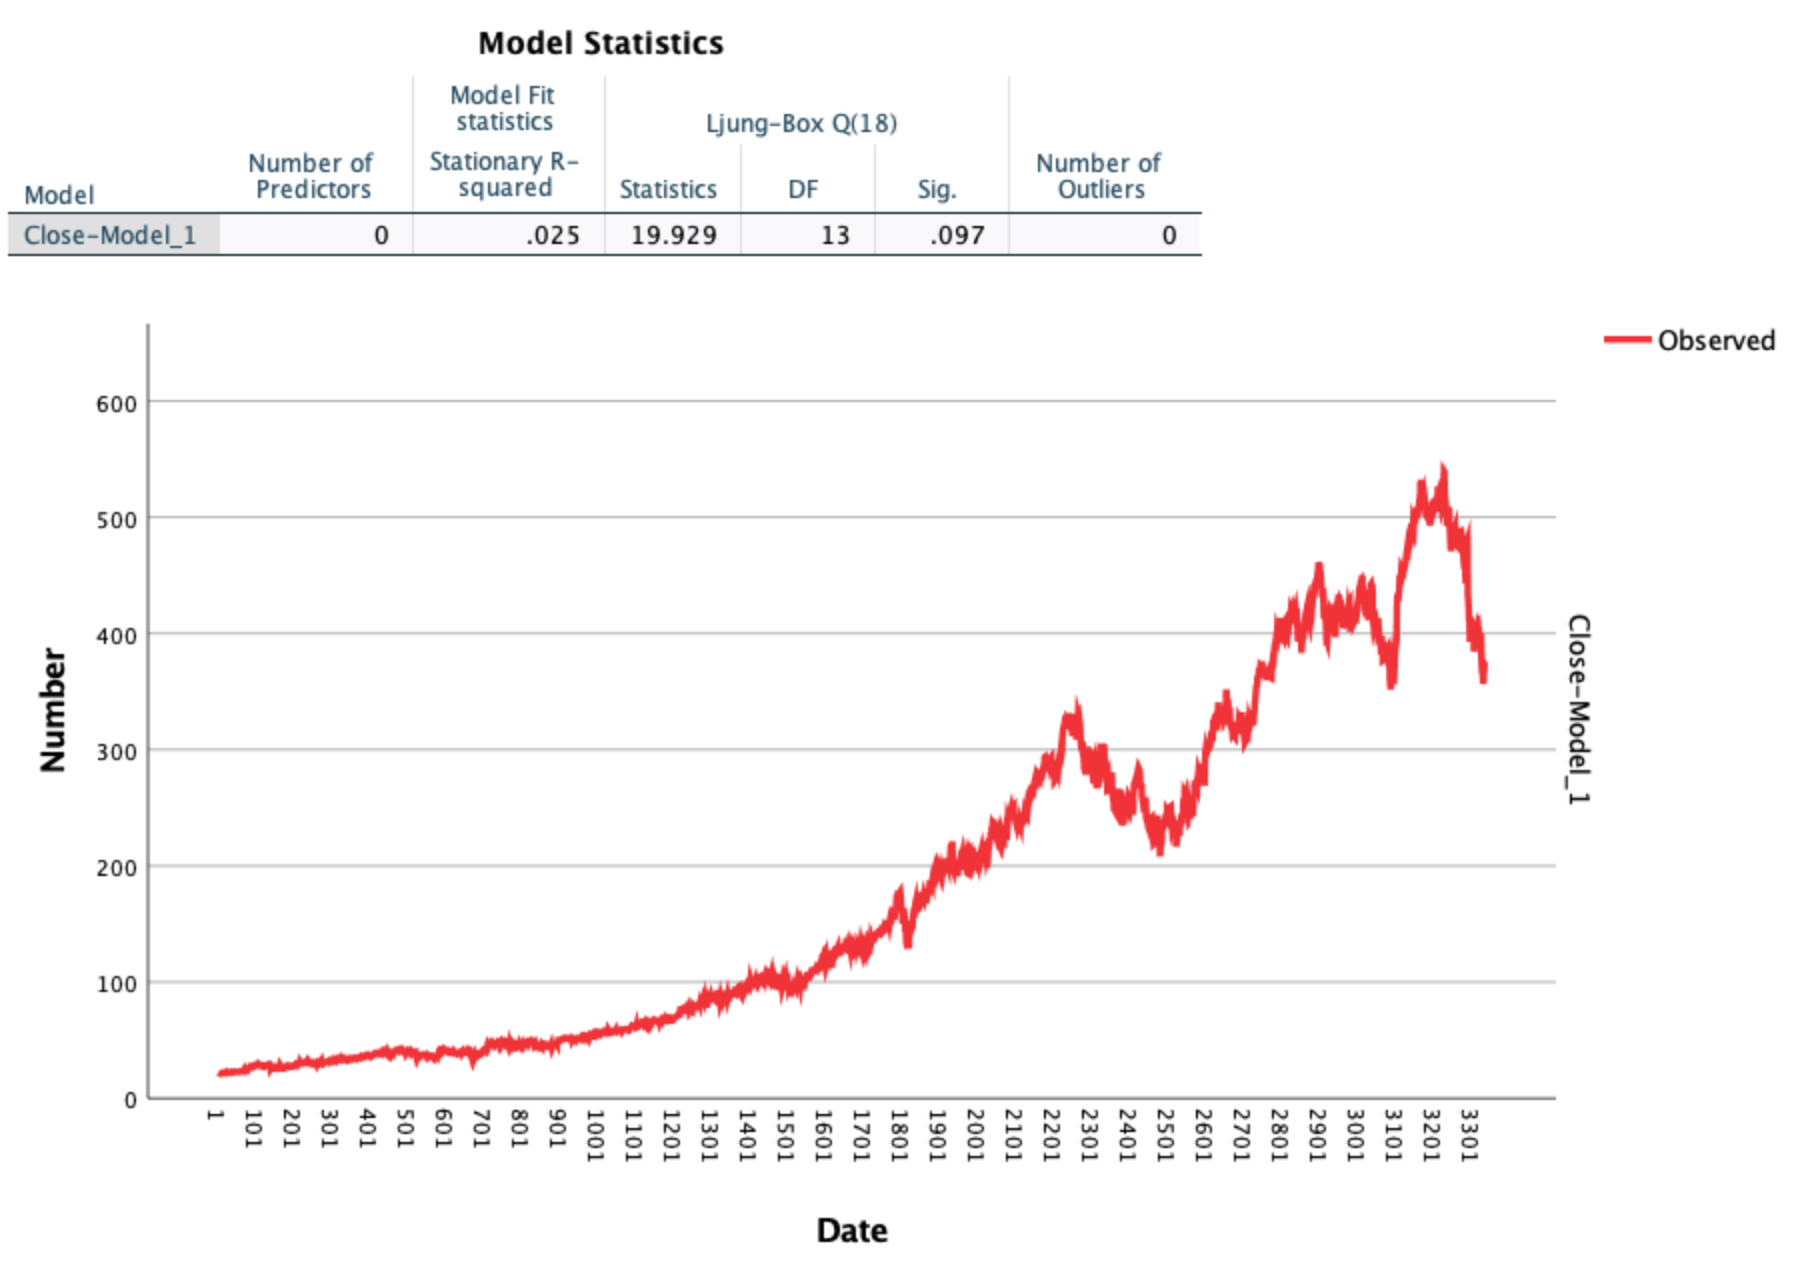
\includegraphics[width=0.95\textwidth]{LAB05/pics/expert_model.png}
    \caption{Mô hình ARIMA(2,1,8) từ Expert Modeler}
\end{figure}

Các chỉ số đánh giá của mô hình:

\begin{itemize}
    \item RMSE = 3.741
    \item MAE = 2.133
    \item MAPE = 1.134\%
\end{itemize}

Kiểm định Ljung-Box cho p-value = 0.097 (> 0.05), cho thấy phần dư không còn tự tương quan. Điều này chứng tỏ mô hình phù hợp hơn về mặt thống kê so với mô hình ban đầu.

\subsection{Kết luận}

Dữ liệu giá cổ phiếu MSFT có xu hướng tăng và không dừng, do đó cần thực hiện sai phân để đảm bảo tính dừng. Mô hình ARIMA(0,1,0) cho kết quả dự báo tốt nhưng chưa xử lý được hoàn toàn tự tương quan của phần dư.

Mô hình ARIMA(2,1,8) được lựa chọn bởi Expert Modeler giúp khắc phục vấn đề này và được xem là mô hình phù hợp hơn. Tuy nhiên, sự cải thiện về độ chính xác dự báo không đáng kể, cho thấy dữ liệu tài chính có tính biến động cao và khó dự báo chính xác.